\documentclass[
  shownotes,
  xcolor={svgnames},
  hyperref={colorlinks,citecolor=DarkBlue,linkcolor=DarkRed,urlcolor=DarkBlue}
  , aspectratio=169]{beamer}
\usepackage{animate}
\usepackage{amsmath}
\usepackage{amsfonts}
\usepackage{amssymb}
\usepackage{pifont}
\usepackage{mathpazo}
%\usepackage{xcolor}
\usepackage{multimedia}
\usepackage{fancybox}
\usepackage[para]{threeparttable}
\usepackage{multirow}
\setcounter{MaxMatrixCols}{30}
\usepackage{subcaption}
\usepackage{graphicx}
\usepackage{lscape}
\usepackage[compatibility=false,font=small]{caption}
\usepackage{booktabs}
\usepackage{ragged2e}
\usepackage{chronosys}
\usepackage{appendixnumberbeamer}
\usepackage{animate}
\setbeamertemplate{caption}[numbered]
\usepackage{color}
%\usepackage{times}
\usepackage{tikz}
\usepackage{comment} %to comment
%% BibTeX settings
\usepackage{natbib}
\bibliographystyle{apalike}
\bibpunct{(}{)}{,}{a}{,}{,}
\setbeamertemplate{bibliography item}{[\theenumiv]}

% Defines columns for bespoke tables
\usepackage{array}
\newcolumntype{L}[1]{>{\raggedright\let\newline\\\arraybackslash\hspace{0pt}}m{#1}}
\newcolumntype{C}[1]{>{\centering\let\newline\\\arraybackslash\hspace{0pt}}m{#1}}
\newcolumntype{R}[1]{>{\raggedleft\let\newline\\\arraybackslash\hspace{0pt}}m{#1}}


\usepackage{xfrac}


\usepackage{multicol}
\setlength{\columnsep}{0.5cm}

% Theme and colors
\usetheme{Boadilla}

% I use steel blue and a custom color palette. This defines it.
\definecolor{andesred}{HTML}{af2433}

% Other options
\providecommand{\U}[1]{\protect\rule{.1in}{.1in}}
\usefonttheme{serif}
\setbeamertemplate{itemize items}[default]
\setbeamertemplate{enumerate items}[square]
\setbeamertemplate{section in toc}[circle]

\makeatletter

\definecolor{mybackground}{HTML}{82CAFA}
\definecolor{myforeground}{HTML}{0000A0}

\setbeamercolor{normal text}{fg=black,bg=white}
\setbeamercolor{alerted text}{fg=red}
\setbeamercolor{example text}{fg=black}

\setbeamercolor{background canvas}{fg=myforeground, bg=white}
\setbeamercolor{background}{fg=myforeground, bg=mybackground}

\setbeamercolor{palette primary}{fg=black, bg=gray!30!white}
\setbeamercolor{palette secondary}{fg=black, bg=gray!20!white}
\setbeamercolor{palette tertiary}{fg=white, bg=andesred}

\setbeamercolor{frametitle}{fg=andesred}
\setbeamercolor{title}{fg=andesred}
\setbeamercolor{block title}{fg=andesred}
\setbeamercolor{itemize item}{fg=andesred}
\setbeamercolor{itemize subitem}{fg=andesred}
\setbeamercolor{itemize subsubitem}{fg=andesred}
\setbeamercolor{enumerate item}{fg=andesred}
\setbeamercolor{item projected}{bg=gray!30!white,fg=andesred}
\setbeamercolor{enumerate subitem}{fg=andesred}
\setbeamercolor{section number projected}{bg=gray!30!white,fg=andesred}
\setbeamercolor{section in toc}{fg=andesred}
\setbeamercolor{caption name}{fg=andesred}
\setbeamercolor{button}{bg=gray!30!white,fg=andesred}



\usepackage{fancyvrb}
\newcommand{\VerbBar}{|}
\newcommand{\VERB}{\Verb[commandchars=\\\{\}]}
\DefineVerbatimEnvironment{Highlighting}{Verbatim}{commandchars=\\\{\}}
% Add ',fontsize=\small' for more characters per line
\usepackage{framed}
\definecolor{shadecolor}{RGB}{248,248,248}
\newenvironment{Shaded}{\begin{snugshade}}{\end{snugshade}}
\newcommand{\AlertTok}[1]{\textcolor[rgb]{0.94,0.16,0.16}{#1}}
\newcommand{\AnnotationTok}[1]{\textcolor[rgb]{0.56,0.35,0.01}{\textbf{\textit{#1}}}}
\newcommand{\AttributeTok}[1]{\textcolor[rgb]{0.77,0.63,0.00}{#1}}
\newcommand{\BaseNTok}[1]{\textcolor[rgb]{0.00,0.00,0.81}{#1}}
\newcommand{\BuiltInTok}[1]{#1}
\newcommand{\CharTok}[1]{\textcolor[rgb]{0.31,0.60,0.02}{#1}}
\newcommand{\CommentTok}[1]{\textcolor[rgb]{0.56,0.35,0.01}{\textit{#1}}}
\newcommand{\CommentVarTok}[1]{\textcolor[rgb]{0.56,0.35,0.01}{\textbf{\textit{#1}}}}
\newcommand{\ConstantTok}[1]{\textcolor[rgb]{0.00,0.00,0.00}{#1}}
\newcommand{\ControlFlowTok}[1]{\textcolor[rgb]{0.13,0.29,0.53}{\textbf{#1}}}
\newcommand{\DataTypeTok}[1]{\textcolor[rgb]{0.13,0.29,0.53}{#1}}
\newcommand{\DecValTok}[1]{\textcolor[rgb]{0.00,0.00,0.81}{#1}}
\newcommand{\DocumentationTok}[1]{\textcolor[rgb]{0.56,0.35,0.01}{\textbf{\textit{#1}}}}
\newcommand{\ErrorTok}[1]{\textcolor[rgb]{0.64,0.00,0.00}{\textbf{#1}}}
\newcommand{\ExtensionTok}[1]{#1}
\newcommand{\FloatTok}[1]{\textcolor[rgb]{0.00,0.00,0.81}{#1}}
\newcommand{\FunctionTok}[1]{\textcolor[rgb]{0.00,0.00,0.00}{#1}}
\newcommand{\ImportTok}[1]{#1}
\newcommand{\InformationTok}[1]{\textcolor[rgb]{0.56,0.35,0.01}{\textbf{\textit{#1}}}}
\newcommand{\KeywordTok}[1]{\textcolor[rgb]{0.13,0.29,0.53}{\textbf{#1}}}
\newcommand{\NormalTok}[1]{#1}
\newcommand{\OperatorTok}[1]{\textcolor[rgb]{0.81,0.36,0.00}{\textbf{#1}}}
\newcommand{\OtherTok}[1]{\textcolor[rgb]{0.56,0.35,0.01}{#1}}
\newcommand{\PreprocessorTok}[1]{\textcolor[rgb]{0.56,0.35,0.01}{\textit{#1}}}
\newcommand{\RegionMarkerTok}[1]{#1}
\newcommand{\SpecialCharTok}[1]{\textcolor[rgb]{0.00,0.00,0.00}{#1}}
\newcommand{\SpecialStringTok}[1]{\textcolor[rgb]{0.31,0.60,0.02}{#1}}
\newcommand{\StringTok}[1]{\textcolor[rgb]{0.31,0.60,0.02}{#1}}
\newcommand{\VariableTok}[1]{\textcolor[rgb]{0.00,0.00,0.00}{#1}}
\newcommand{\VerbatimStringTok}[1]{\textcolor[rgb]{0.31,0.60,0.02}{#1}}
\newcommand{\WarningTok}[1]{\textcolor[rgb]{0.56,0.35,0.01}{\textbf{\textit{#1}}}}
\usepackage{graphicx}
\makeatletter

\makeatother


%%%%%%%%%%%%%%% BEGINS DOCUMENT %%%%%%%%%%%%%%%%%%

\begin{document}

\title{Lecture 3:  Regularizacion y Clasificacion}
\subtitle{Aprendizaje y Minería de Datos para los Negocios}
\date{\today}

\author[Sarmiento-Barbieri]{Ignacio Sarmiento-Barbieri}
\institute[Uniandes]{Universidad de los Andes}


\begin{frame}[noframenumbering]
\maketitle
\end{frame}

%%%%%%%%%%%%%%%%%%%%%%%%%%%%%%%%%%%
%       Motivation              %
% What is the question?
% Why do we care?
% What is new?
% What do you find?
%%%%%%%%%%%%%%%%%%%%%%%%%%%%%%%%%%%




\begin{frame}
\frametitle{Agenda}

\tableofcontents


\end{frame}
%----------------------------------------------------------------------%
\section{Recap} 
%----------------------------------------------------------------------%
%----------------------------------------------------------------------%
\subsection{Predicción} 
%----------------------------------------------------------------------%
%----------------------------------------------------------------------%
\begin{frame}
\frametitle{Predicción y Error Predictivo}


\begin{itemize}
  \item El objetivo es predecir $y$ dadas otras variables $X$. 
  \bigskip
  \item Asumimos que el link entre $y$ and $X$ esta dado por el modelo:
\end{itemize}
\bigskip
\begin{align}
  y = f(X) + u
\end{align}
\bigskip
\begin{itemize}
  \item donde $f(X)$ es cualquier función, 
  \bigskip
  \item  $u$ una variable aleatoria no observable $E(u)=0$ and $V(u) = \sigma^2$
\end{itemize}


\end{frame}

%----------------------------------------------------------------------%
\begin{frame}
\frametitle{Predicción y Error Predictivo}

\begin{itemize}
  \item En la práctica no conocemos $f(X)$
  \medskip
  \item Es necesario estimarla $\hat y = \hat f(X)$ 
  \medskip
  \item La medida de cuan bien funciona nuestro modelo es 
    \begin{align}
      MSE(y)= \frac{1}{n} \sum_{i=1}^n (y_i - \hat{y}_i )^2
    \end{align}
  
  \item Notemos que podemos descomponer el $MSE$ en dos partes
\end{itemize}

\begin{align}
  MSE (  y )  &= MSE(\hat f) + \sigma^2  \\  
  &= Bias^2(\hat f) + V(\hat f) +  \sigma^2
\end{align}

\begin{itemize}
  \item  el error de estimar $f$ con $\hat f$. (\emph{reducible})
  \item  el error de no observar $u$, $\sigma^2$. (\emph{irreducible})
  \item  dilema entre sesgo y varianza
\end{itemize}

\medskip

\end{frame}



%----------------------------------------------------------------------%
\subsection{Overfit}
%----------------------------------------------------------------------%

%----------------------------------------------------------------------%
\begin{frame}<1>[label=overfit]
\frametitle{Overfit y Predicción fuera de Muestra}


\begin{itemize}
  \item ML nos interesa la predicción fuera de muestra
  \medskip
  \item Overfit: modelos complejos predicen muy bien dentro de muestra, pero tienden a hacer un trabajo fuera de muestra 
  \pause
  \medskip
  \item Hay que elegir el modelo que ``mejor'' prediga
  \medskip

    \begin{itemize}
    \item Medidas Clásicas
      \scriptsize
      \begin{align}
      AIC(j) &= log \left( \frac{1}{n} \sum_{i=1}^n (y_i - \hat{y}_i )^2\right)- p_j \\
      SIC(j) &= log \left( \frac{1}{n} \sum_{i=1}^n (y_i - \hat{y}_i )^2\right) -  p_j \frac{1}{2} log(n)
      \end{align}

    \item Métodos de Remuestreo
      \begin{itemize}
      \item Validación cruzada en K-partes (5 o 10)
      \item Usar el MSE
      \end{itemize}
    \end{itemize}

\end{itemize}

\end{frame}
%----------------------------------------------------------------------%
\begin{frame}[fragile, noframenumbering]
\frametitle{Overfit}


        \begin{figure}[H] \centering
            \captionsetup{justification=centering}
              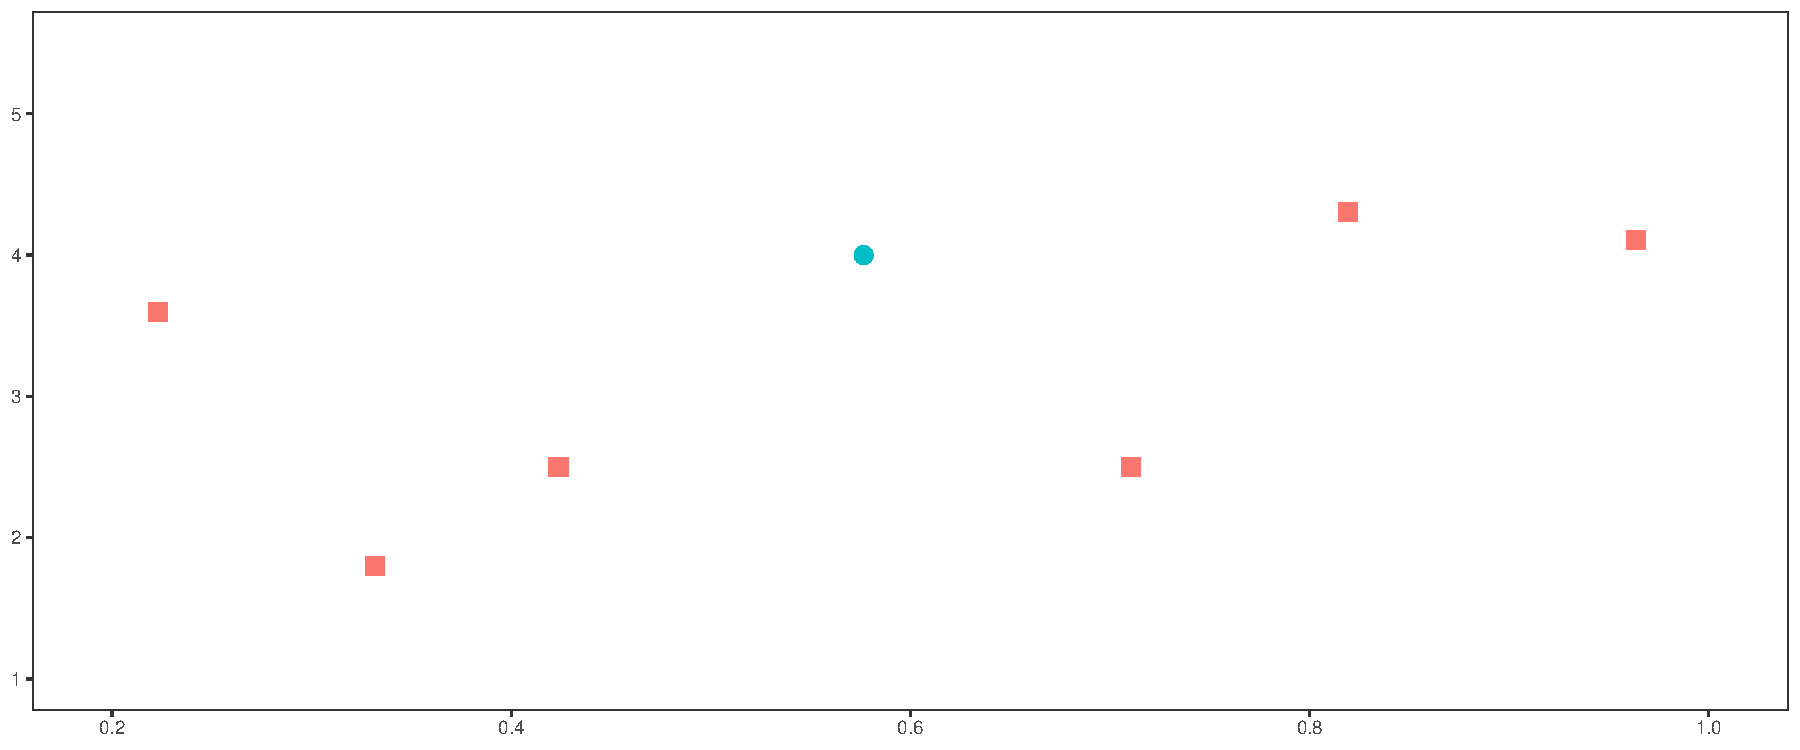
\includegraphics[scale=0.4]{figures/fig_1g.pdf}
 \end{figure}

\end{frame}
%----------------------------------------------------------------------%
\begin{frame}[fragile, noframenumbering]
\frametitle{Overfit}


        \begin{figure}[H] \centering
            \captionsetup{justification=centering}
              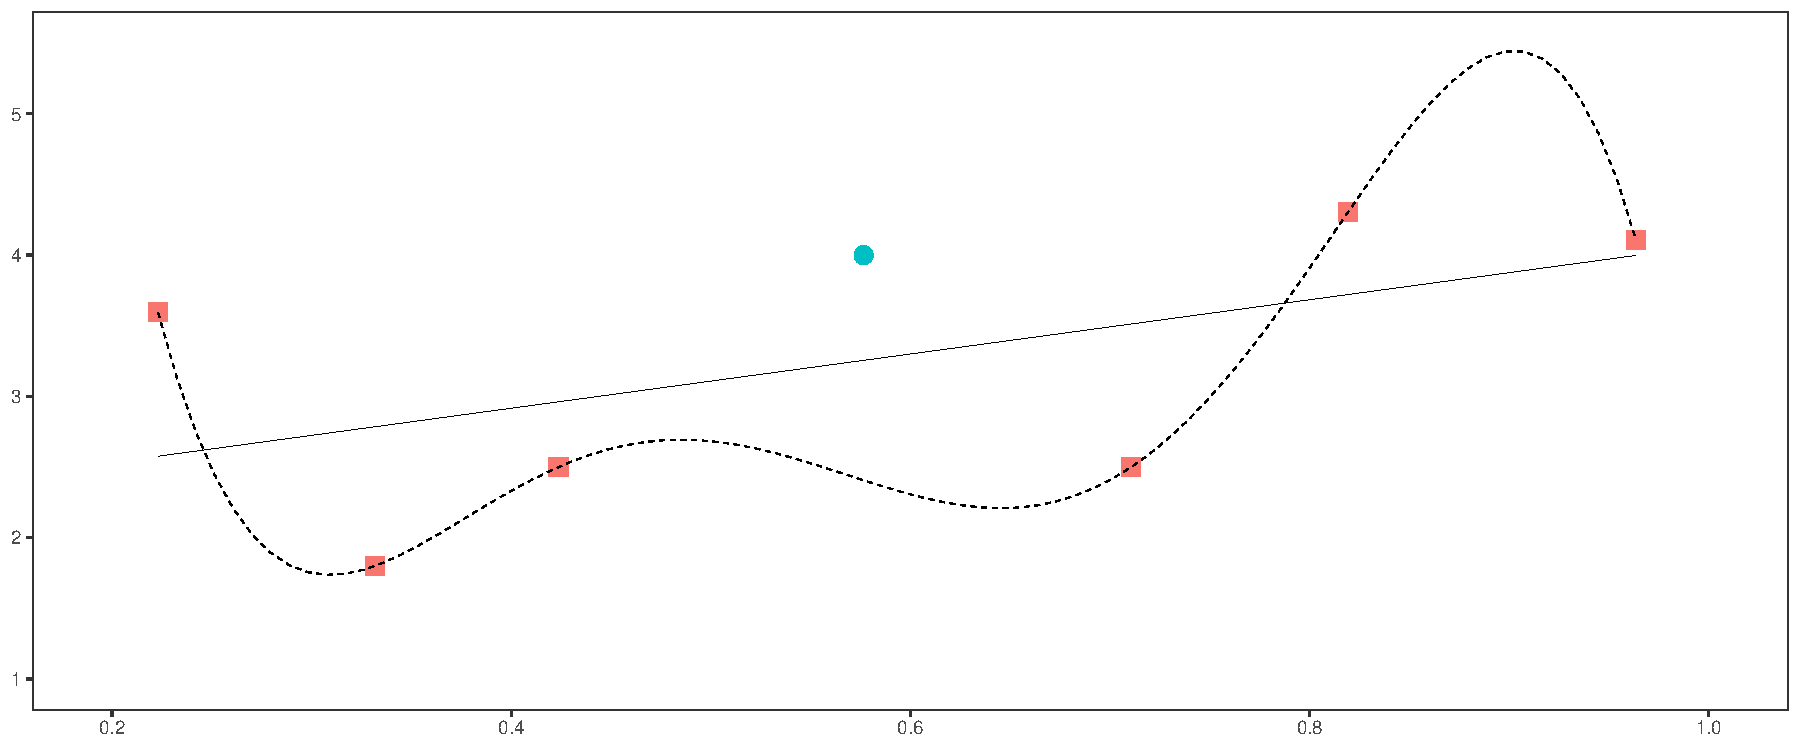
\includegraphics[scale=0.4]{figures/fig_1h.pdf}
 \end{figure}

\end{frame}
%----------------------------------------------------------------------%
\againframe<2>{overfit}

%----------------------------------------------------------------------%
\section{Regularización}
%----------------------------------------------------------------------%

\begin{frame}[fragile]
\frametitle{}


\centering
{\huge \textcolor{andesred}{Regularización}}



\end{frame}

%----------------------------------------------------------------------%
\subsection{Lasso}
%----------------------------------------------------------------------%
\begin{frame}[fragile]
\frametitle{Lasso}

\begin{itemize}
\item Para un $\lambda \geq 0$ dado, consideremos el siguiente problema de optimización


\begin{align}
min_{\beta} E(\beta) = \sum_{i=1}^n (y_i-\beta_0 - x_{i1}\beta_1 - \dots - x_{ip}\beta_p)^2 + \lambda \sum_{j=1}^p |\beta_j| 
\end{align}

\medskip
\pause
  \begin{itemize}
    \item  ``LASSO's free lunch'': selecciona automáticamente los predictores que van en el modelo ($\beta_j \neq 0$) y los que no   ($\beta_j = 0$)
    \medskip
    \item Porque? Los coeficientes que no van son soluciones de esquina
    \medskip
    \item  $L(\beta)$ es no differentiable
  \end{itemize}
\end{itemize}

\end{frame}
%----------------------------------------------------------------------%
\begin{frame}[fragile]
\frametitle{Lasso Intuición en 1 Dimension}

\begin{itemize}
\item Lasso Intuición
\end{itemize}

\bigskip

\begin{align}
min_{\beta} E(\beta) = \sum_{i=1}^n (y_i-x_i \beta)^2 + \lambda|\beta| 
\end{align}

\begin{itemize}
  \item Un solo predictor, un solo coeficiente
  \medskip
  \item Si $\lambda=0$
\begin{align}
  min_{\beta} E(\beta) = \sum_{i=1}^n (y_i-x_i \beta)^2 
  \end{align}
  \item y la solución es
  \begin{align}
    \hat{\beta}_{OLS}
  \end{align}
  
\end{itemize}

\end{frame}
%----------------------------------------------------------------------%
\begin{frame}[fragile]
\frametitle{Intuición en 1 Dimension}

\begin{align}
 min_{\beta} E(\beta) = \sum_{i=1}^n (y_i-x_i \beta)^2 + \lambda|\beta| 
\end{align}
   \begin{figure}[H] \centering
            \captionsetup{justification=centering}
              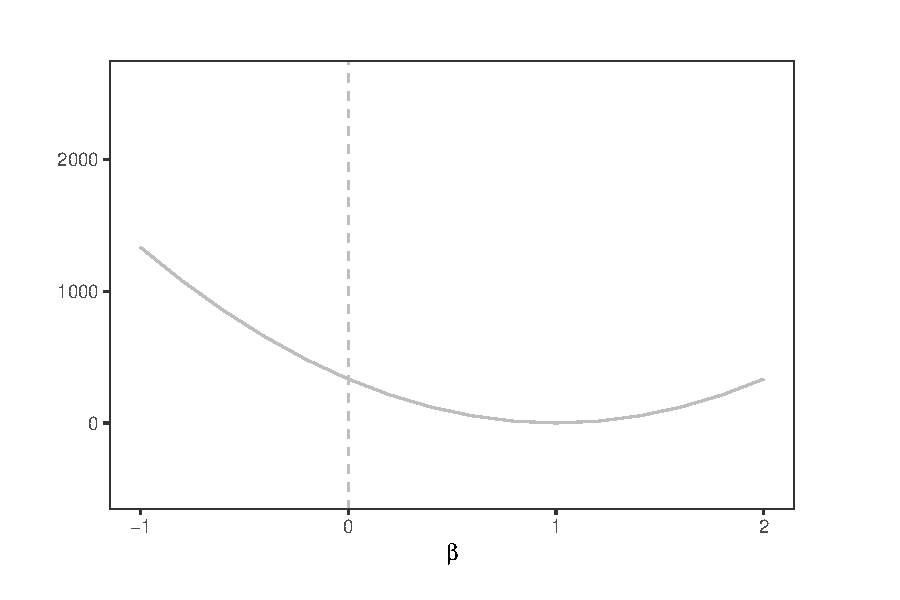
\includegraphics[scale=0.6]{figures/lasso0.pdf}
 \end{figure}



\end{frame}
%----------------------------------------------------------------------%
\begin{frame}[fragile]
\frametitle{Intuición en 1 Dimension}

\begin{align}
 min_{\beta} E(\beta) = \sum_{i=1}^n (y_i-x_i \beta)^2 + \lambda|\beta| 
\end{align}
   \begin{figure}[H] \centering
            \captionsetup{justification=centering}
              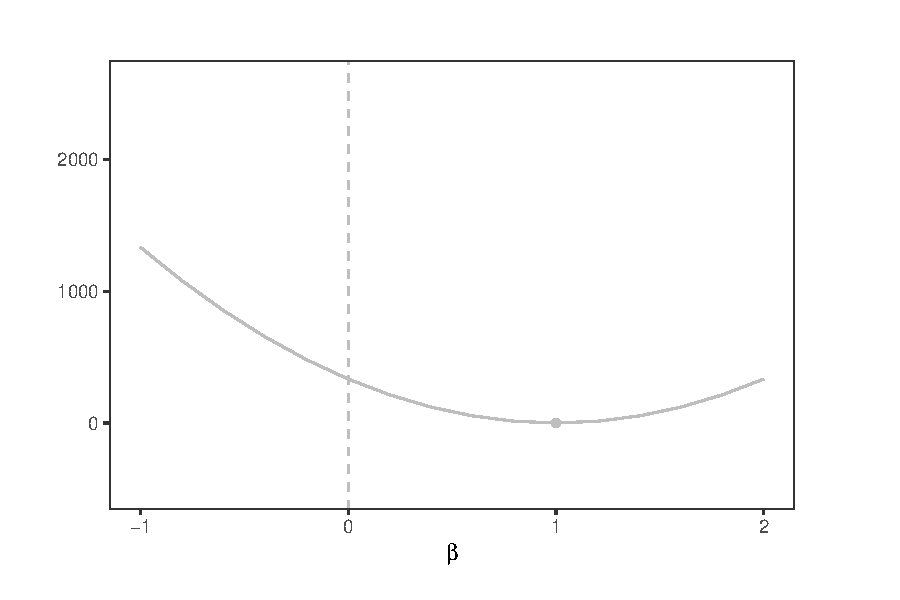
\includegraphics[scale=0.6]{figures/lasso1.pdf}
 \end{figure}




\end{frame}
%----------------------------------------------------------------------%
\begin{frame}[fragile]
\frametitle{Intuición en 1 Dimension}

\begin{align}
 min_{\beta} E(\beta) = \sum_{i=1}^n (y_i-x_i \beta)^2 + \lambda|\beta| 
\end{align}
   \begin{figure}[H] \centering
            \captionsetup{justification=centering}
              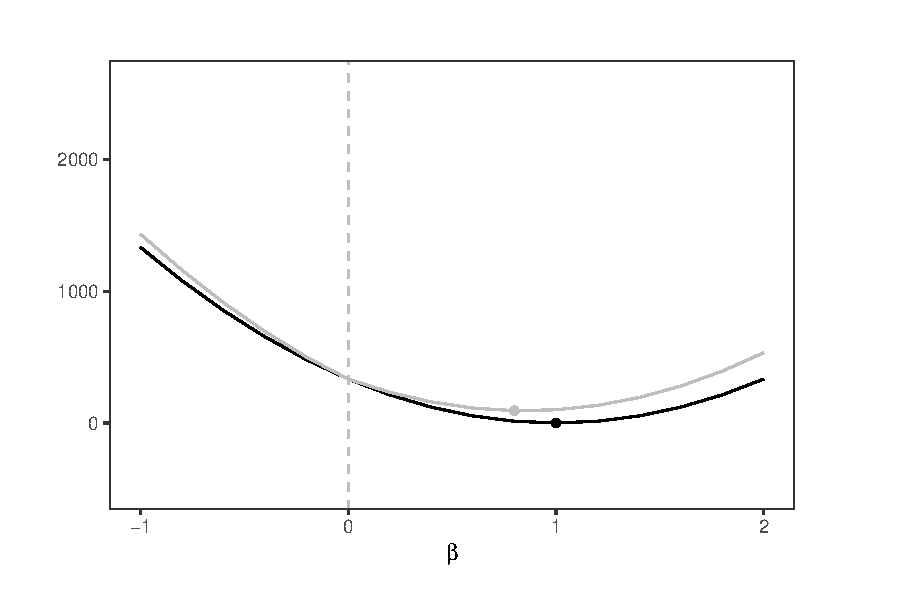
\includegraphics[scale=0.6]{figures/lasso2.pdf}
 \end{figure}




\end{frame}
%----------------------------------------------------------------------%
\begin{frame}[fragile]
\frametitle{Intuición en 1 Dimension}

\begin{align}
 min_{\beta} E(\beta) = \sum_{i=1}^n (y_i-x_i \beta)^2 + \lambda|\beta| 
\end{align}

   \begin{figure}[H] \centering
            \captionsetup{justification=centering}
              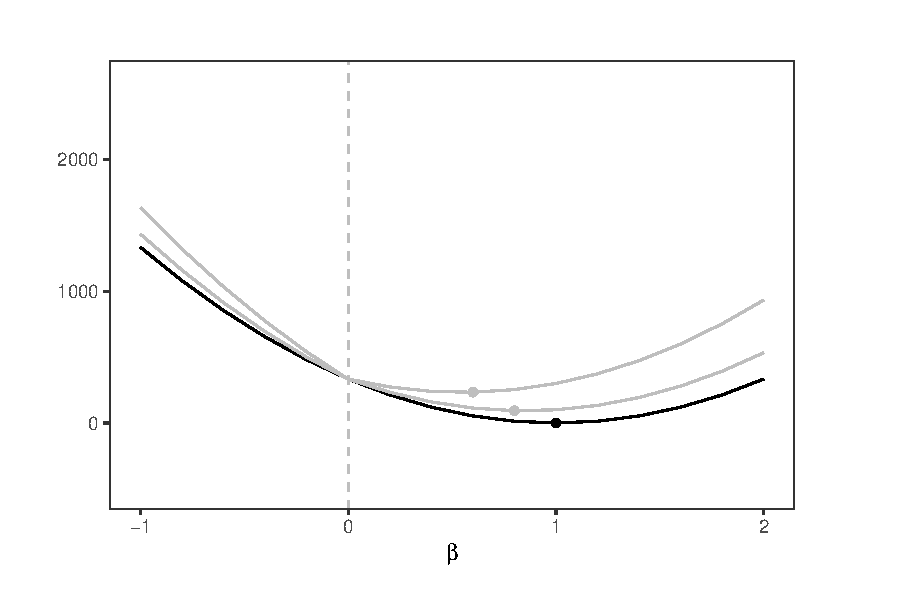
\includegraphics[scale=0.6]{figures/lasso3.pdf}
 \end{figure}




\end{frame}
%----------------------------------------------------------------------%
\begin{frame}[fragile]
\frametitle{Intuición en 1 Dimension}

\begin{align}
 min_{\beta} E(\beta) = \sum_{i=1}^n (y_i-x_i \beta)^2 + \lambda|\beta| 
\end{align}

   \begin{figure}[H] \centering
            \captionsetup{justification=centering}
              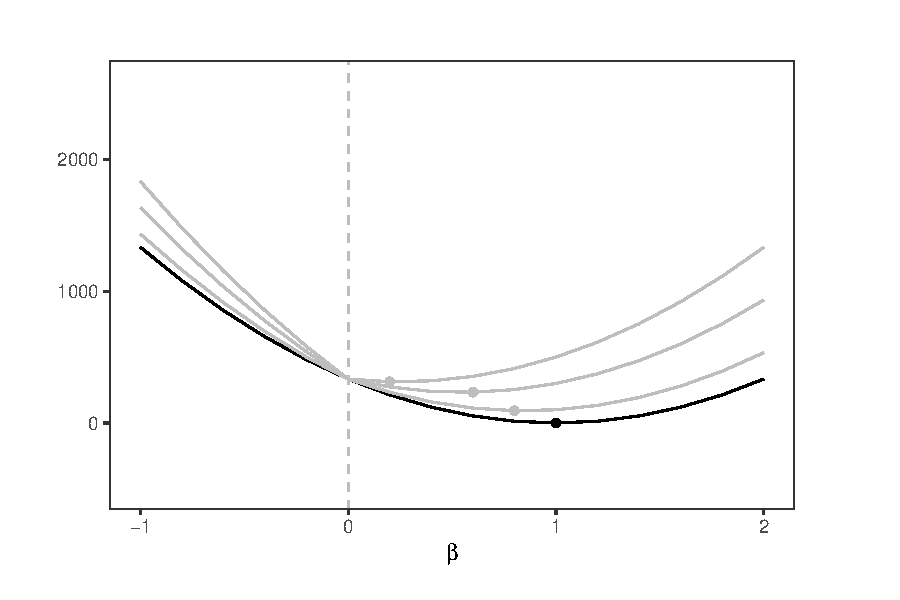
\includegraphics[scale=0.6]{figures/lasso4.pdf}
 \end{figure}





\end{frame}
%----------------------------------------------------------------------%
\begin{frame}[fragile]
\frametitle{Intuición en 1 Dimension}

\begin{align}
 min_{\beta} E(\beta) = \sum_{i=1}^n (y_i-x_i \beta)^2 + \lambda|\beta| 
\end{align}

   \begin{figure}[H] \centering
            \captionsetup{justification=centering}
              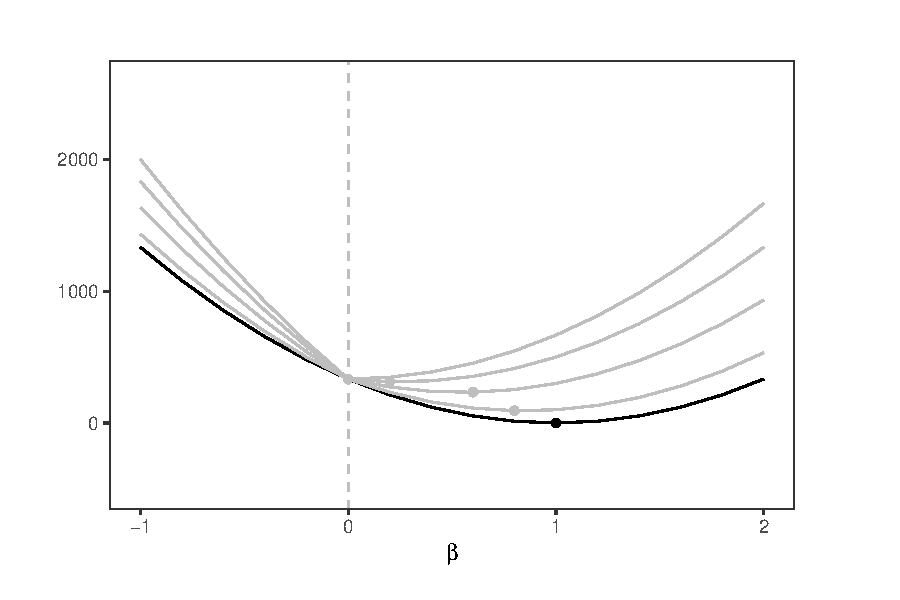
\includegraphics[scale=0.6]{figures/lasso5.pdf}
 \end{figure}


\end{frame}
%----------------------------------------------------------------------%
\begin{frame}[fragile]
\frametitle{Intuición en 1 Dimension}

\begin{align}
 min_{\beta} E(\beta) = \sum_{i=1}^n (y_i-x_i \beta)^2 + \lambda|\beta| 
\end{align}

   \begin{figure}[H] \centering
            \captionsetup{justification=centering}
              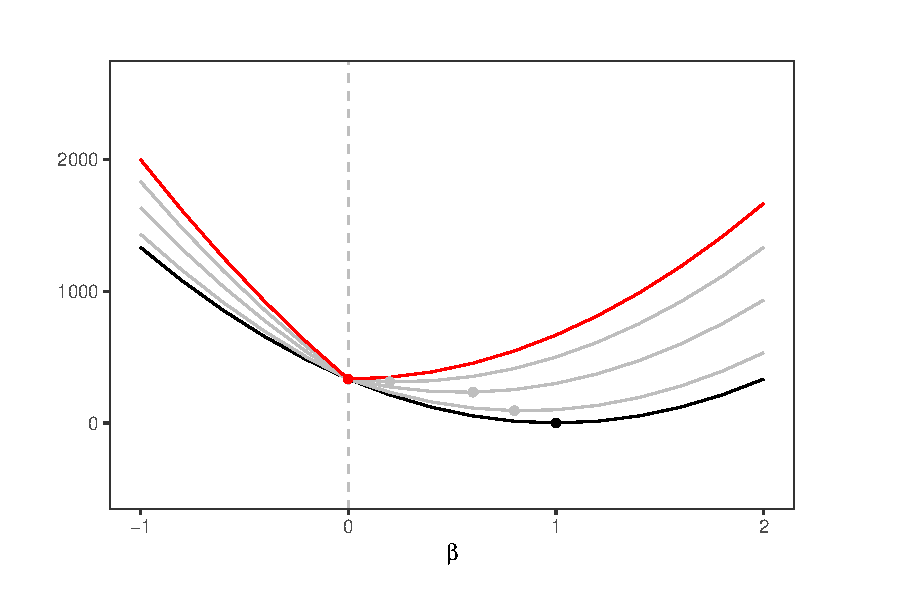
\includegraphics[scale=0.6]{figures/lasso6.pdf}
 \end{figure}


\end{frame}
%----------------------------------------------------------------------%
\begin{frame}[fragile]
\frametitle{Intuición en 1 Dimension}

\begin{align}
 min_{\beta} E(\beta) = \sum_{i=1}^n (y_i-x_i \beta)^2 + \lambda|\beta| 
\end{align}

   \begin{figure}[H] \centering
            \captionsetup{justification=centering}
              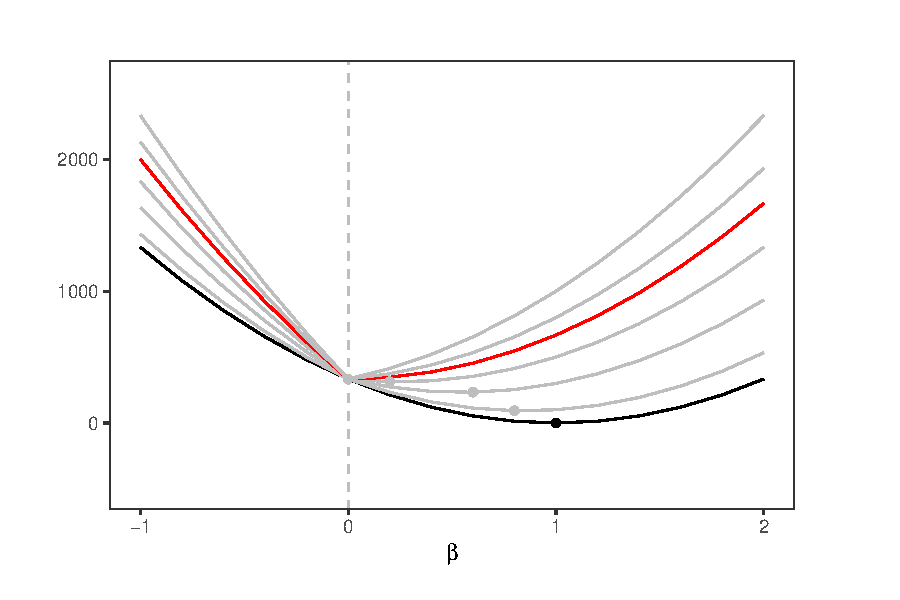
\includegraphics[scale=0.6]{figures/lasso_final.pdf}
 \end{figure}

 \end{frame}

%----------------------------------------------------------------------%
\begin{frame}[fragile]
\frametitle{Intuición en 1 Dimension}

\begin{align}
min_{\beta} E(\beta) = \sum_{i=1}^n (y_i-x_i \beta)^2 + \lambda|\beta| 
\end{align}

la solución analítica es 
\medskip
\begin{align}
\hat{\beta}_{lasso}=\begin{cases}
0 & \text{\text{si} }\ensuremath{\lambda\geq \lambda^*}\\
\hat{\beta}_{OLS}-\frac{\lambda}{2} & \text{\text{si} }\ensuremath{\lambda<\lambda^*}
\end{cases}
\end{align}



 \end{frame}
%----------------------------------------------------------------------%
\subsection{Ridge}
%----------------------------------------------------------------------%
\begin{frame}[fragile]
\frametitle{Ridge}

\begin{itemize}
\item Para un $\lambda \geq 0$ dado, consideremos ahora el siguiente problema de optimización


\begin{align}
min_{\beta} E(\beta) = \sum_{i=1}^n (y_i-\beta_0 - x_{i1}\beta_1 - \dots - x_{ip}\beta_p)^2 + \lambda \sum_{j=1}^p (\beta_j)^2
\end{align}

\bigskip
\item La intuición es similar a lasso, pero la vamos a extender a 2-Dim

\end{itemize}


\end{frame}
%----------------------------------------------------------------------%
\begin{frame}[fragile]
\frametitle{Intuición en 2 Dimensiones (OLS)}

\begin{align}
min_{\beta} E(\beta) = \sum_{i=1}^n (y_i - x_{i1}\beta_1 - x_{i1}\beta_2)^2 
\end{align}
\begin{figure}[H] \centering
            \captionsetup{justification=centering}
              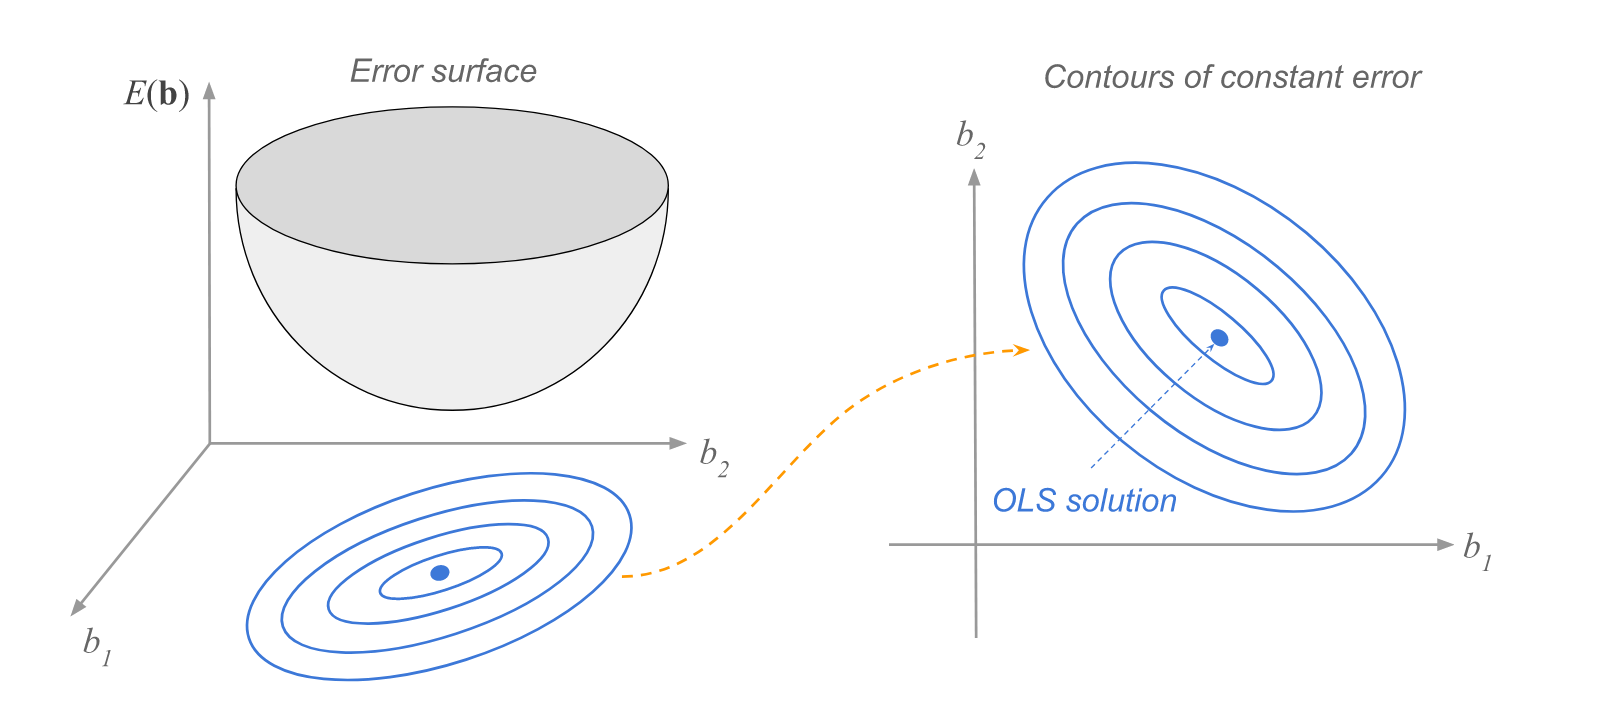
\includegraphics[scale=0.3]{figures/ols1}
 
\tiny
Fuente: \url{https://allmodelsarewrong.github.io}
\end{figure}


\end{frame}
%----------------------------------------------------------------------%
\begin{frame}[fragile]
\frametitle{Intuición en 2 Dimensiones (OLS)}

\begin{align}
min_{\beta} E(\beta) = \sum_{i=1}^n (y_i - x_{i1}\beta_1 - x_{i1}\beta_2)^2 
\end{align}

\begin{figure}[H] \centering
            \captionsetup{justification=centering}
              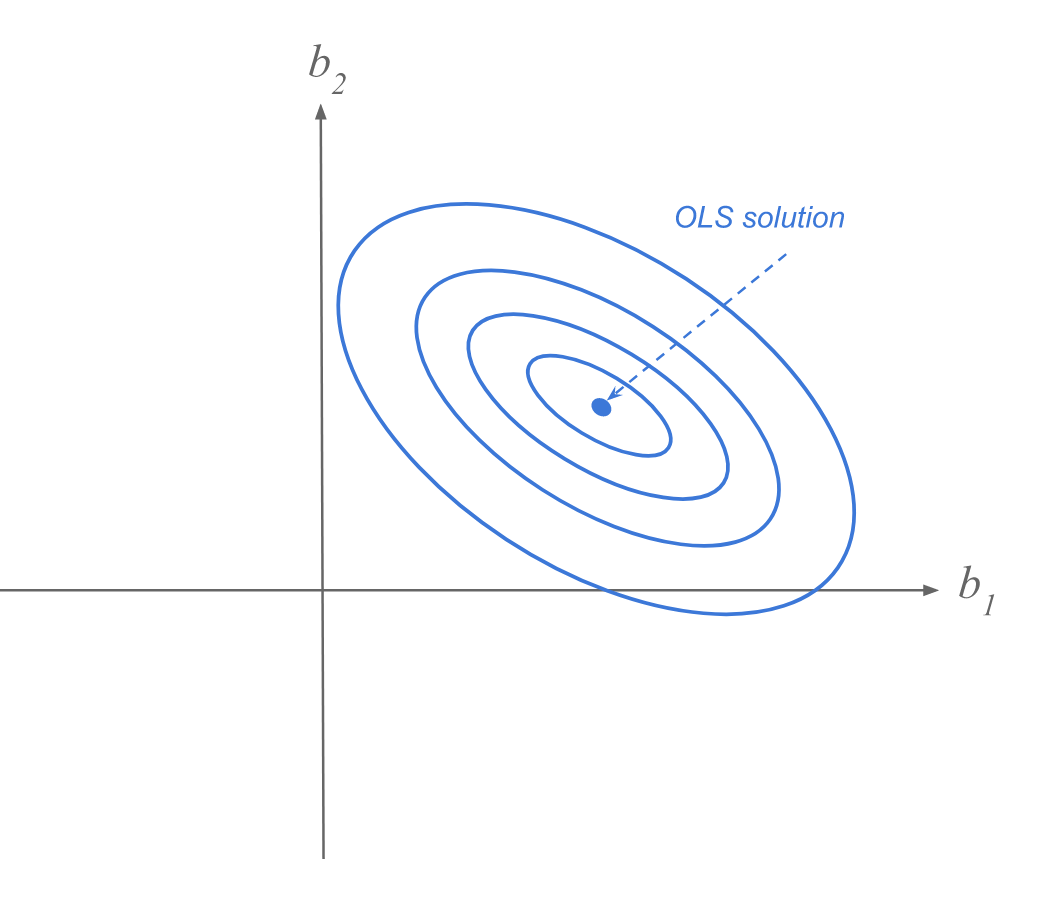
\includegraphics[scale=0.3]{figures/ols2}
 
\tiny
Fuente: \url{https://allmodelsarewrong.github.io}
\end{figure}


\end{frame}
%----------------------------------------------------------------------%
\begin{frame}[fragile]
\frametitle{Intuición en 2 Dimensiones (Ridge)}

\begin{itemize}
\item Al problema

  \begin{align}
  min_{\beta} E(\beta) = \sum_{i=1}^n (y_i-\beta_0 - x_{i1}\beta_1 - \dots - x_{ip}\beta_p)^2 + \lambda \sum_{j=1}^p (\beta_j)^2
  \end{align}
\medskip 
\item podemos escribirlo como
  \begin{align}
     min_{\beta} E(\beta) &= \sum_{i=1}^n (y_i - x_{i1}\beta_1 - x_{i1}\beta_2)^2  \\ \nonumber
     & \text{sujeto a}   \\
     & \left( (\beta_1)^2 + (\beta_2)^2 \right) \leq c \nonumber
  \end{align}

\end{itemize}

\end{frame}
%----------------------------------------------------------------------%
\begin{frame}[fragile]
\frametitle{Intuición en 2 Dimensiones (Ridge)}

\begin{align}
     min_{\beta} E(\beta) &= \sum_{i=1}^n (y_i - x_{i1}\beta_1 - x_{i1}\beta_2)^2  \text{ s.a }   \left( (\beta_1)^2 + (\beta_2)^2 \right) \leq c 
  \end{align}

\begin{figure}[H] \centering
            \captionsetup{justification=centering}
              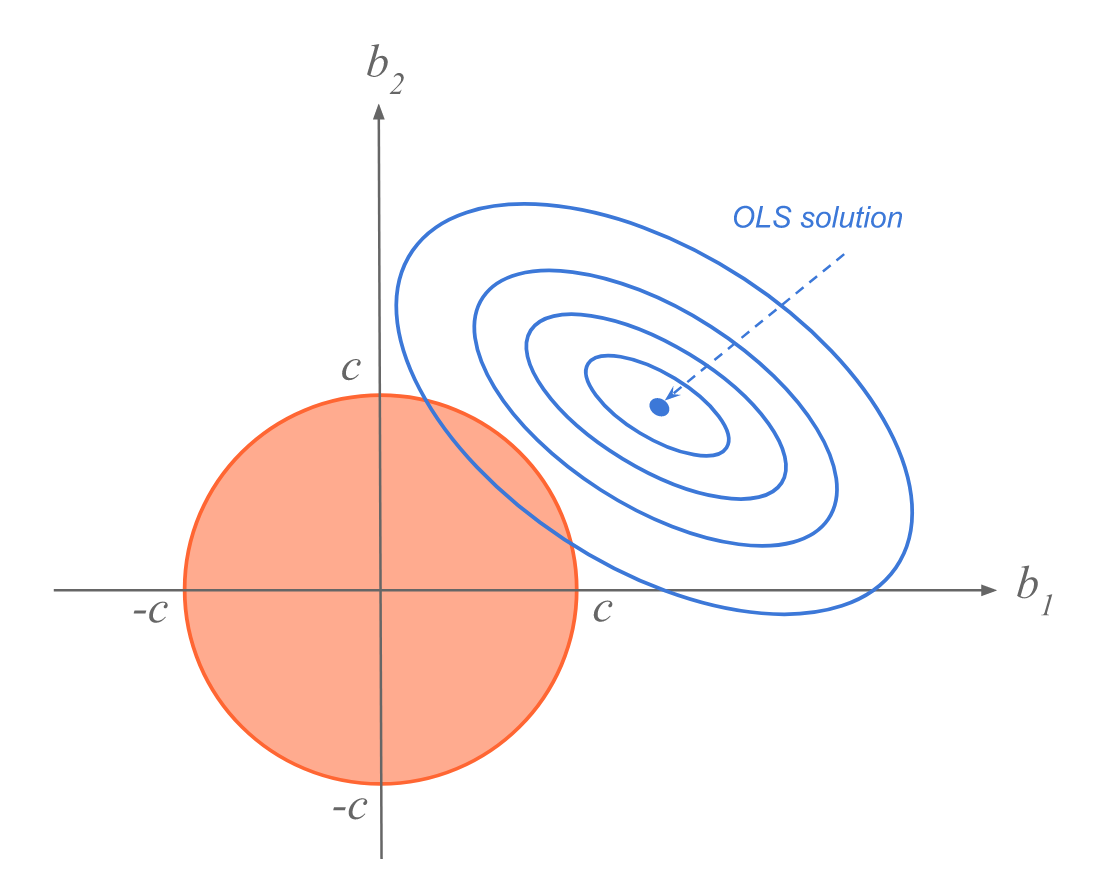
\includegraphics[scale=0.3]{figures/ridge1}
 
\tiny
Fuente: \url{https://allmodelsarewrong.github.io}
\end{figure}


\end{frame}
%----------------------------------------------------------------------%
\begin{frame}[fragile]
\frametitle{Intuición en 2 Dimensiones (Ridge)}

\begin{align}
     min_{\beta} E(\beta) &= \sum_{i=1}^n (y_i - x_{i1}\beta_1 - x_{i1}\beta_2)^2  \text{ s.a }   \left( (\beta_1)^2 + (\beta_2)^2 \right) \leq c 
  \end{align}

\begin{figure}[H] \centering
            \captionsetup{justification=centering}
              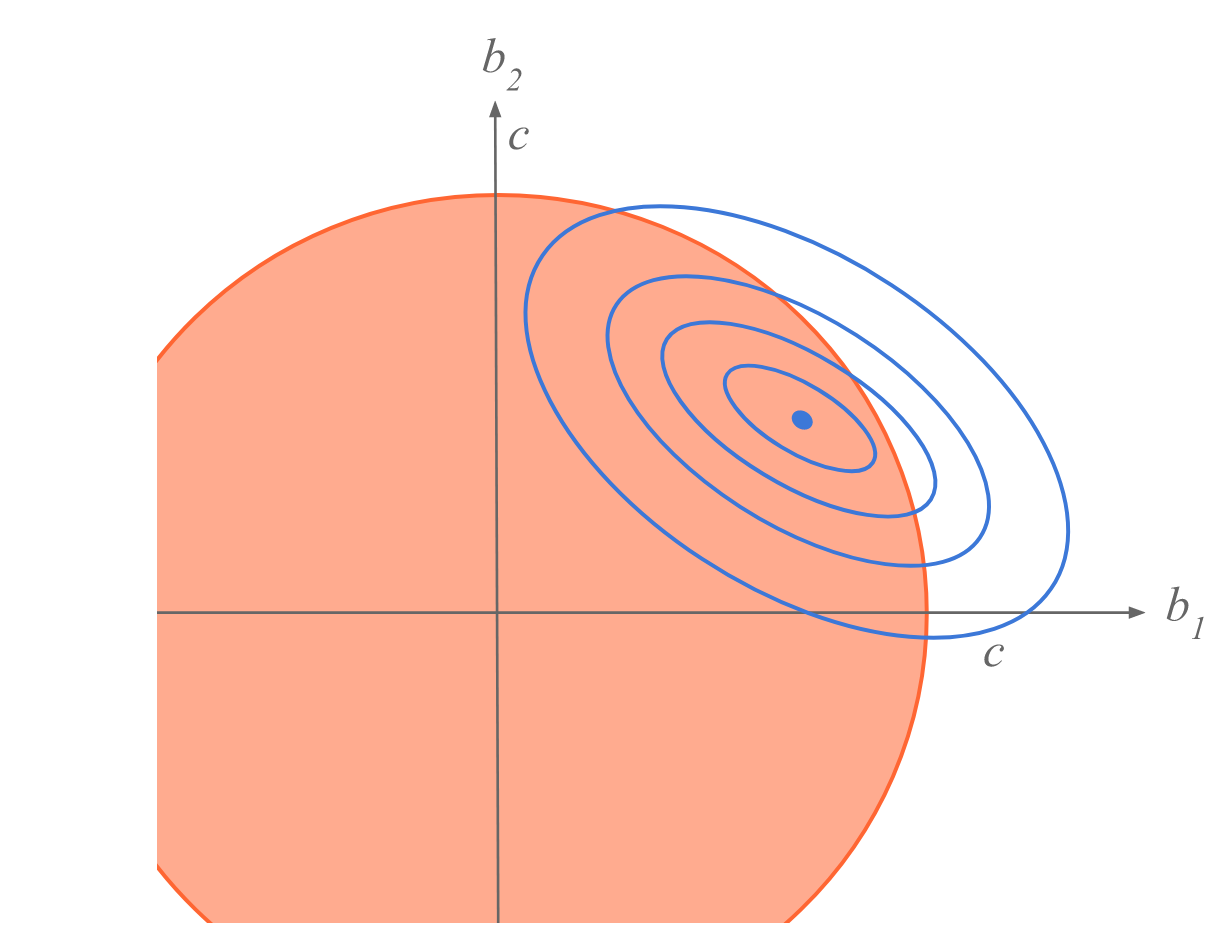
\includegraphics[scale=0.3]{figures/ridge2}
 
\tiny
Fuente: \url{https://allmodelsarewrong.github.io}
\end{figure}


\end{frame}
%----------------------------------------------------------------------%
\begin{frame}[fragile]
\frametitle{Intuición en 2 Dimensiones (Ridge)}

\begin{align}
     min_{\beta} E(\beta) &= \sum_{i=1}^n (y_i - x_{i1}\beta_1 - x_{i1}\beta_2)^2  \text{ s.a }   \left( (\beta_1)^2 + (\beta_2)^2 \right) \leq c 
  \end{align}

\begin{figure}[H] \centering
            \captionsetup{justification=centering}
              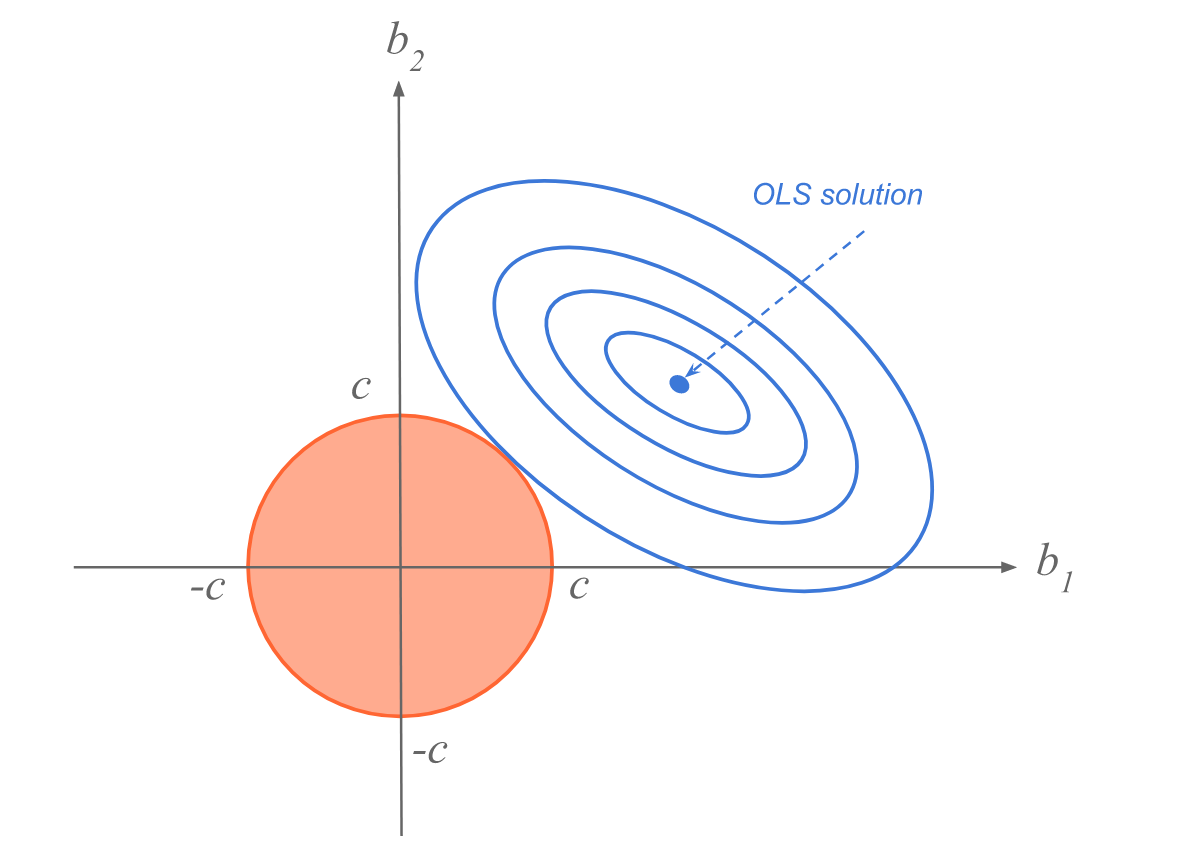
\includegraphics[scale=0.3]{figures/ridge3}
 
\tiny
Fuente: \url{https://allmodelsarewrong.github.io}
\end{figure}


\end{frame}
%----------------------------------------------------------------------%
\begin{frame}[fragile]
\frametitle{Intuición en 2 Dimensiones (Ridge)}

\begin{align}
     min_{\beta} E(\beta) &= \sum_{i=1}^n (y_i - x_{i1}\beta_1 - x_{i1}\beta_2)^2  \text{ s.a }   \left( (\beta_1)^2 + (\beta_2)^2 \right) \leq c 
  \end{align}

\begin{figure}[H] \centering
            \captionsetup{justification=centering}
              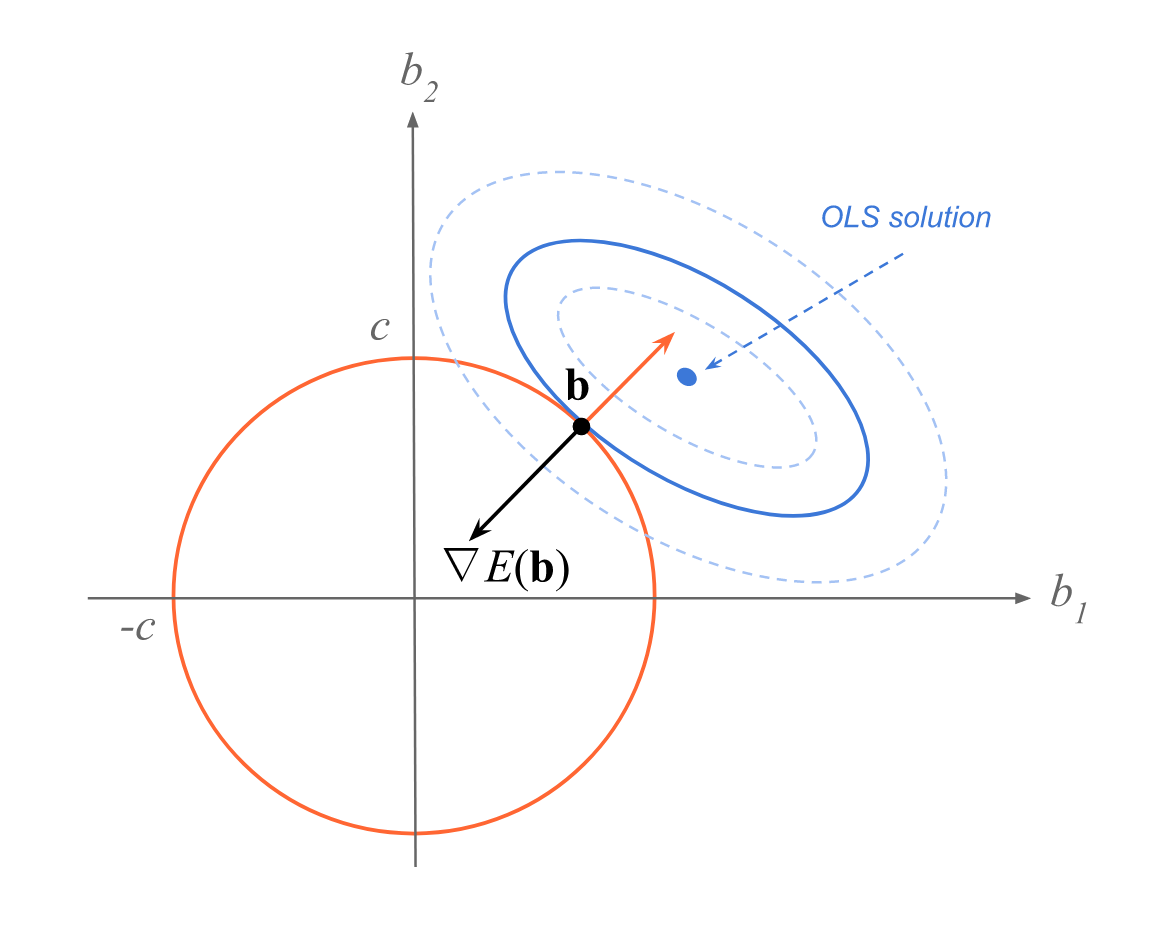
\includegraphics[scale=0.3]{figures/ridge4}
 
\tiny
Fuente: \url{https://allmodelsarewrong.github.io}
\end{figure}


\end{frame}
%----------------------------------------------------------------------%
\begin{frame}[fragile]
\frametitle{Intuición en 2 Dimensiones (Lasso)}

\begin{align}
     min_{\beta} E(\beta) &= \sum_{i=1}^n (y_i - x_{i1}\beta_1 - x_{i1}\beta_2)^2  \text{ s.a }   \left( |\beta_1| + |\beta_2| \right) \leq c 
  \end{align}

\begin{figure}[H] \centering
            \captionsetup{justification=centering}
              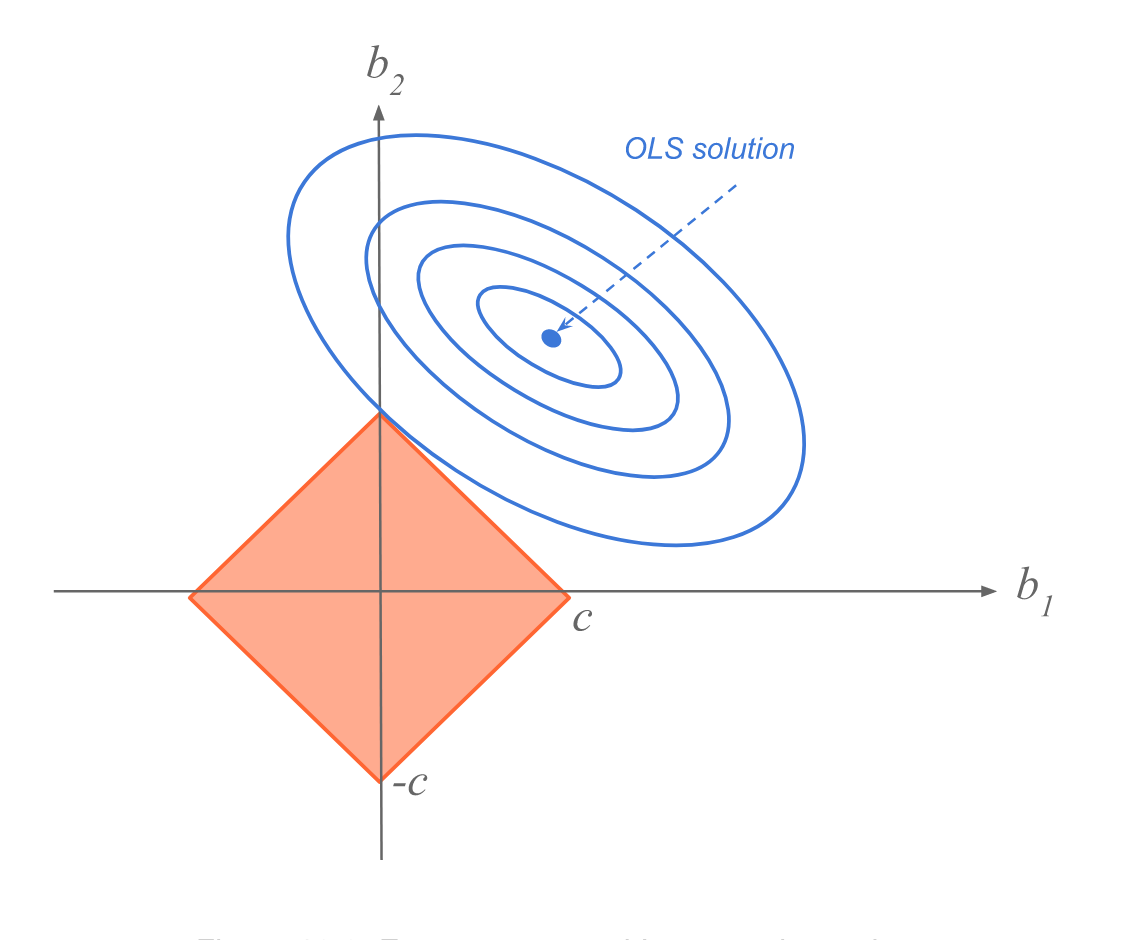
\includegraphics[scale=0.4]{figures/lasso_ridge2}
 
\tiny
Fuente: \url{https://allmodelsarewrong.github.io}
\end{figure}




\end{frame}
%----------------------------------------------------------------------%
\begin{frame}[fragile]
\frametitle{Lasso y Ridge Ejemplo}

   \begin{figure}[H] \centering
            \captionsetup{justification=centering}
              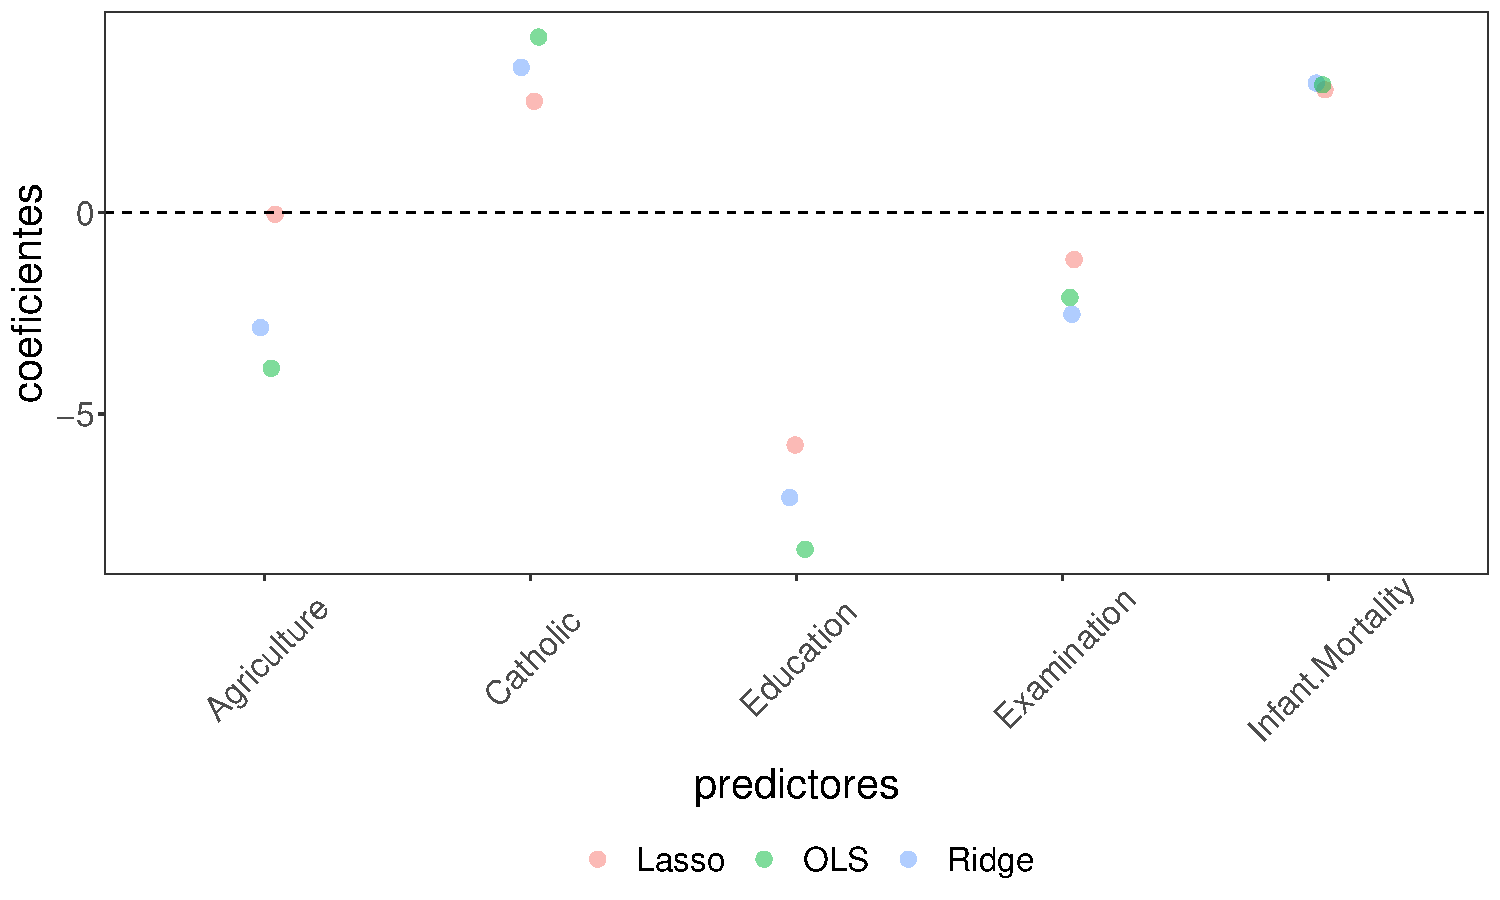
\includegraphics[scale=0.5]{figures/comp}
 \end{figure}

 \end{frame}
%----------------------------------------------------------------------%
\begin{frame}[fragile]
\frametitle{Comentarios técnicos}

\begin{itemize}
 \item Lasso y ridge son sesgados, pero las disminuciones en varianza pueden compensar estoy y llevar a un MSE menor
 \medskip

 \item Lasso encoje a cero, Ridge no tanto
 \medskip
 \item Importante para aplicación:
\begin{itemize}
  \medskip
 \item Estandarizar los datos (media 0, y varianza 1)
 \medskip
 \item Como elegimos $\lambda$?
\end{itemize}
\end{itemize}

 \end{frame}
%----------------------------------------------------------------------%
\begin{frame}[fragile]
\frametitle{Comentarios técnicos: selección de $\lambda$ }
\begin{itemize}
 \item Como elegimos $\lambda$?
 \item $\lambda$ es un parámetro y lo elegimos usando validación cruzada

 \begin{enumerate}
 \item Partimos la muestra de entrenamiento en K Partes: $M_{train}= M_{fold\,1} \cup M_{fold\,2} \dots \cup M_{fold\,K}$
 \item Cada conjunto  $M_{fold\,K}$ va a jugar el rol de una muestra de evaluación $M_{eval\,k}$. Entonces para cada muestra
 \begin{itemize}
  \item  $M_{train-1}=M_{train} - M_{fold\,1}$
  \item  $\vdots$
  \item  $M_{train-k}=M_{train} - M_{fold\,k}$
 \end{itemize}
 \item Luego hacemos el siguiente loop
 \begin{enumerate}
 \item Para $\lambda_i=0,0.001,0.002,\dots,\lambda_{max}$ \\
      - Para $k=1,\dots,K$ \\
      $\,\,\,\,\,\,$- Ajustar el modelo $m_{i,k}$ con $\lambda_i$ en $M_{train-k}$ \\
      $\,\,\,\,\,\,$- Calcular y guardar el $MSE(m_{i,k})$ usando $M_{eval-k}$ \\
      - fin para k \\
      - Calcular y guardar $MSE_i=\frac{1}{K} MSE(m_{i,k})$ \\
\item fin para $\lambda$
 \end{enumerate}
 \item Encontrar el menor $MSE_i$ y usar ese $\lambda_i=\lambda^*$
  \end{enumerate}
\end{itemize}

\end{frame}


%----------------------------------------------------------------------%
\section{Classification}
%----------------------------------------------------------------------%
%----------------------------------------------------------------------%
\begin{frame}[fragile]
\frametitle{Classification}


\centering
{\huge \textcolor{andesred}{Classification}}



\end{frame}
%----------------------------------------------------------------------%
\begin{frame}[fragile]
\frametitle{Classification: Motivation}

\begin{itemize}
  \item Muchas de las preguntas predictivas suelen ser de clasificación
  \medskip
  \pause
  \item Predecir si un usuario va a hacer click o no
  \medskip
  \item Decidir si alguien va a ``default'' el credito
  \medskip
  \item La afiliación política basado en los discursos
  \medskip
  \item La diferencia es que ahora $y$ representa la pertenencia a una clase
  \medskip
  \item $y\in \{0,1,\dots,m\}$ 
    \begin{quote}
      La pregunta es: dado un nuevo conjunto de predictores $X$ es nuestra mejor predicción de la categoría a la que pertenece  
    \end{quote}
\end{itemize}



\end{frame}

%----------------------------------------------------------------------%
\subsection{K vecinos cercanos (KNN)}
%----------------------------------------------------------------------%
%----------------------------------------------------------------------%
\begin{frame}[fragile]
\frametitle{K vecinos cercanos (KNN)}

\begin{itemize}
\item K vecinos cercanos predice la clase $\hat y$ a partir de $x$ preguntandose \\
{\it Cual es la clase mas común para la observarción alrededor x?}
\end{itemize}
        \begin{figure}[H] \centering
            \captionsetup{justification=centering}
              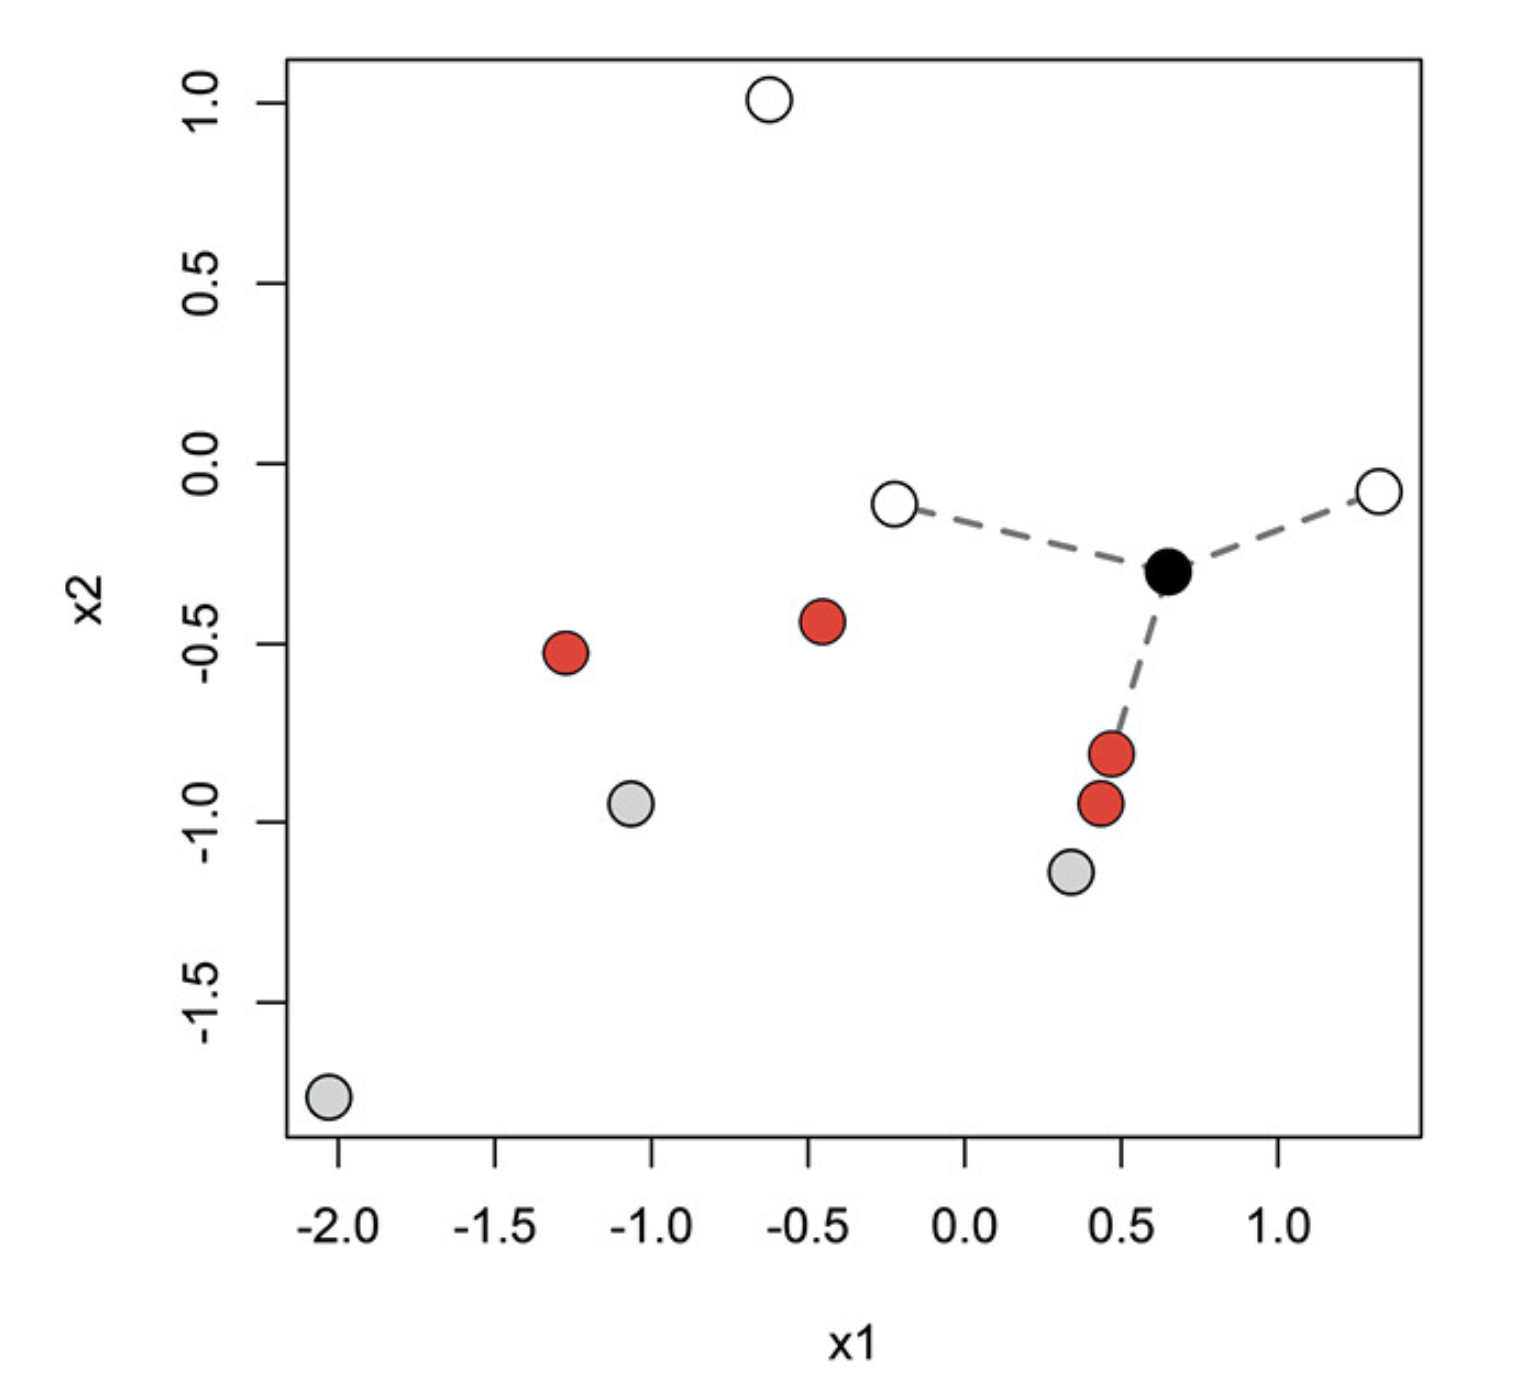
\includegraphics[scale=0.13]{figures/knn}
              \\
              \tiny
              Source: Taddy (2019)
 \end{figure}

 \end{frame}
%----------------------------------------------------------------------%
\begin{frame}[fragile]
\frametitle{K vecinos cercanos (KNN)}

\begin{itemize}
\item K vecinos cercanos predice la clase $\hat y$ a partir de $x$ preguntandose \\
{\it Cual es la clase mas común para la observarción alrededor x?}
\item Algoritmo: dado el insumo  $x_f$ donde nos gustaría la clase:

\begin{itemize}
  \item Encontrar los K vecnos mas cercanos, donde cercanos lo definimos a partir de una distancia, la más común es la euclideana
  \begin{align}
  d(x_i,x_f)=\sqrt{\sum_{j=1}^p(x_{ij}-x_{fj})^2}
  \end{align}
  \item Esto nos da los K vecinos cercanos:
  \begin{align}
  [x_{i1},y_{i1}],\dots,[x_{iK},y_{iK}]
  \end{align}
  \item La clase predicha es la más común
  \begin{align}
  \hat{y}_f =mode\{y_{i1},\dots,y_{iK}\}
  \end{align}
\end{itemize}

\end{itemize}
\end{frame}

%----------------------------------------------------------------------%
\begin{frame}[fragile]
\frametitle{K vecinos cercanos (KNN)}
\begin{itemize}
  \item Hay algunos problemas en aplicaciones
  \medskip
  \begin{itemize}
  \item Las predicciones son inestables como función de $K$
    \end{itemize}
\end{itemize}
  \begin{columns}[T] % align columns
\begin{column}{.58\textwidth}
\begin{align}
  K&=1 \implies \hat{p}(white)=0 \nonumber \\
  K&=2 \implies \hat{p}(white)=1/2 \nonumber \\
  K&=3 \implies \hat{p}(white)=2/3 \nonumber \\
  K&=4 \implies \hat{p}(white)=1/2 \nonumber 
  \end{align}


\end{column}
\hfill
\begin{column}{.4\textwidth}
\begin{figure}[H] \centering
            \captionsetup{justification=centering}
              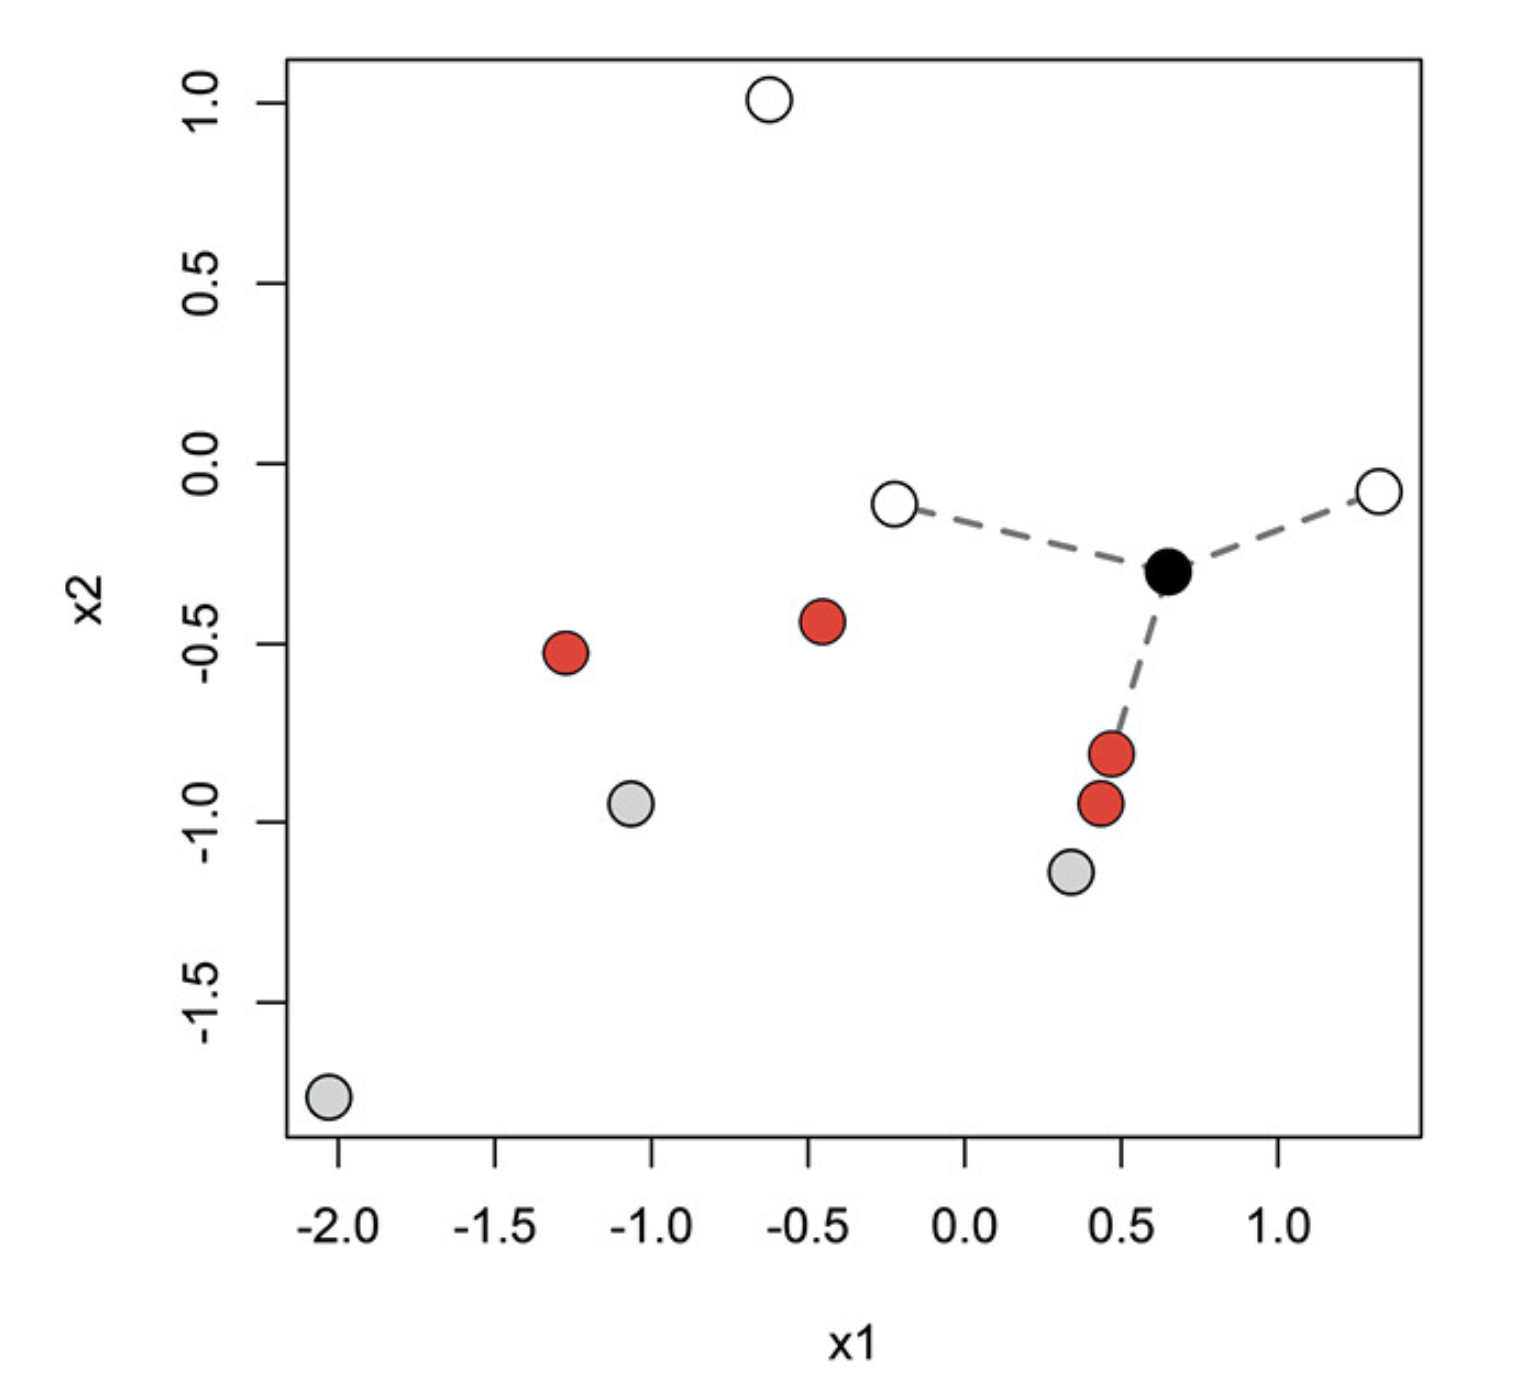
\includegraphics[scale=0.1]{figures/knn}
              \\
              \tiny
              Source: Taddy (2019)
 \end{figure}
\end{column}
\end{columns}
  
\end{frame}


%----------------------------------------------------------------------%
\begin{frame}[fragile]
\frametitle{K vecinos cercanos (KNN)}
\begin{itemize}

  \item Hay algunos problemas en aplicaciones
  \medskip
  \begin{itemize}
  \item Las predicciones son inestables como función de $K$
  \medskip
  \item Esto hace que sea muy dificil elegir el K optimo y validación cruzada no funciona muy bien
  \medskip
  \item Dado que cada predicción  $x$ requiere un proceso de cuenta computacionalmente muy costoso, KNN no es muy util cuando trabajamos con Big Data
  \medskip
  \item KNN es una buena idea, pero demasiado crudo para ser util en la practica
  \end{itemize}
\end{itemize}

\end{frame}


%----------------------------------------------------------------------%
\begin{frame}[fragile]
\frametitle{Probabilidades, Costos, y Clasificación}
\pause
\begin{itemize}
  \item Dos estados de la naturaleza $y \rightarrow n\in\{0,1\}$
  \medskip
  \item Dos acciones $(\hat{y}) \rightarrow a\in \{0,1\}$
  \medskip
  \item Los aciertos y errores que cometemos al clasificar podemos resumirlos en
\end{itemize}
        \begin{figure}[H] \centering
            \captionsetup{justification=centering}
              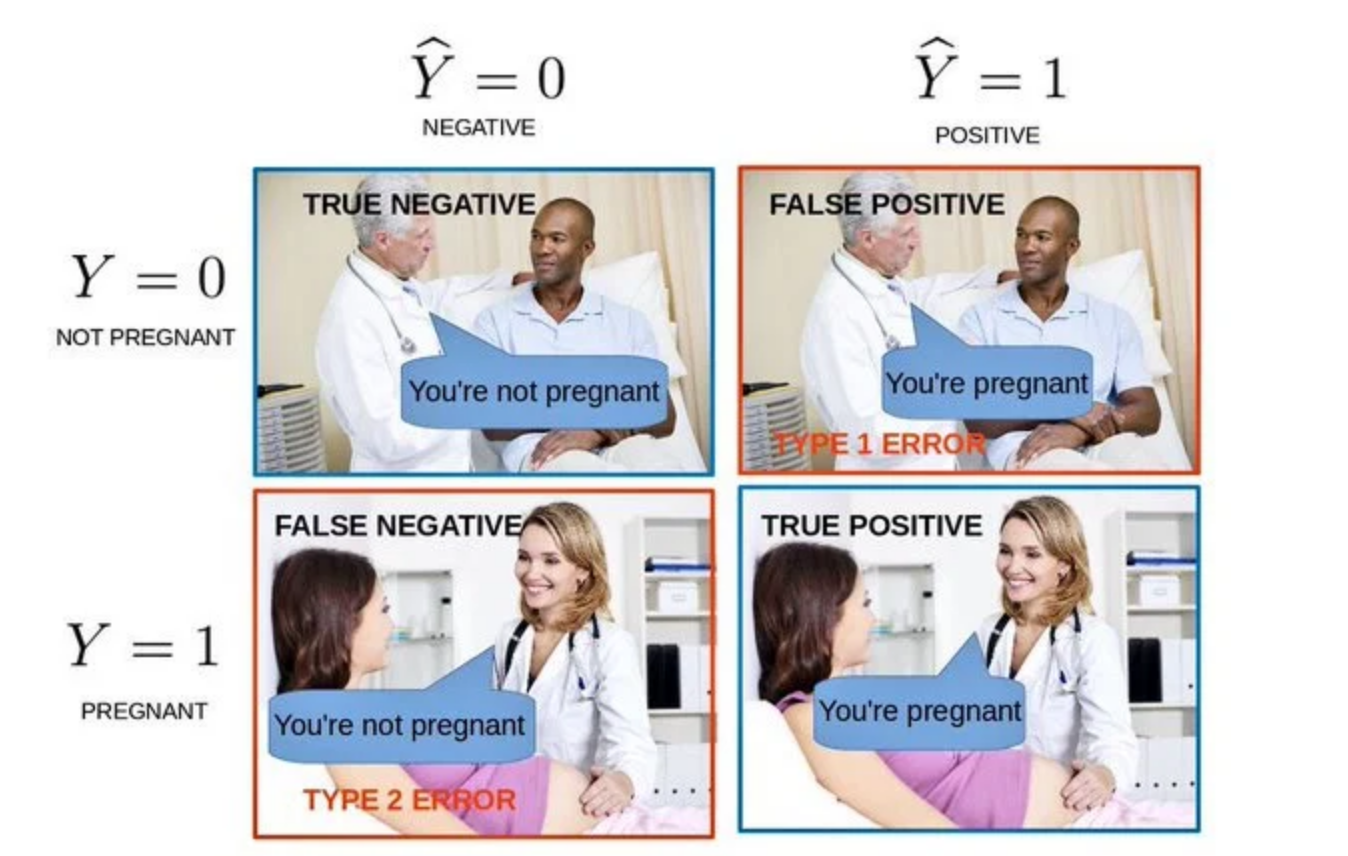
\includegraphics[scale=0.3]{figures/confusion_matrix}
              \\
              \tiny
              Source: \url{https://dzone.com/articles/understanding-the-confusion-matrix}
 \end{figure}


 \end{frame}

%----------------------------------------------------------------------%
\begin{frame}[fragile]
\frametitle{Probabilidades, Costos, y Clasificación}

\begin{itemize}
  \item Dos estados de la naturaleza $y \rightarrow n\in\{0,1\}$
  \medskip
  \item Dos acciones $(\hat{y}) \rightarrow a\in \{0,1\}$
  \medskip
  \item Probabilities
  \begin{itemize}
    \item $p=Pr(y=1|X)$
    \item $1-p=Pr(y=0|X)$
  \end{itemize}
  \medskip
  \item Las acciones tienen costos
  \item y estas puede haber distintos costos asociados 

\end{itemize}


\end{frame}
%----------------------------------------------------------------------%
\begin{frame}[fragile]
\frametitle{Probabilidades, Costos, y Clasificación}

\begin{itemize}
  \item Para tomar una decisión optima, necesitamos estimar las probabilidades de los resultados posibles
  \medskip
  \item Estas probabilidades son las que permiten evaluar la perdida esperada
  \medskip
  \item La perdida esperada por tomar la accion $a$ es

\medskip
\begin{align}
E[Loss(a)] &= \sum_n p_n L(a,n) \\ \nonumber
\end{align}


  \item Al conocer las probabilidades de los distintos resultados podemos evaluar la perdida esperada
  
\end{itemize}
\end{frame}
%----------------------------------------------------------------------%
\begin{frame}[fragile]
\frametitle{Probabilidades, Costos, y Clasificación}

\begin{itemize}
  \item Afortunadamente sabemos como estimar probabilidades
  \medskip
  \begin{itemize}
    \item K-vecinos cercanos
    \item Modelo logístico
    \item entre otras
  \end{itemize}
\medskip
  %\item Hay un trade-off cada vez que elegimos una regla de classificación.
\end{itemize}


\end{frame}

%----------------------------------------------------------------------%
\subsection{Logit}
%----------------------------------------------------------------------%

\begin{frame}[fragile]
\frametitle{Logit}

\begin{itemize}
  \item Podemos modelar la relación entre $p(X)$ y $X$

    \begin{align}
    Pr(y=1|X) &= f(X'\beta) 
    \end{align}

  \item usando la función logística  (sigmoid, softmax) 

  \begin{align}
  p(y=1|X)=\frac{e^{X'\beta}}{1+e^{X'\beta}}=\frac{exp(\beta_0 +\beta_1 x_1 + \dots +\beta_k x_k)}{1+exp(\beta_0 +\beta_1 x_1 + \dots +\beta_k x_k)}
  \end{align}
\end{itemize}
\end{frame}
%----------------------------------------------------------------------%
\begin{frame}[fragile]
\frametitle{Logit}



        \begin{figure}[H] \centering
            \captionsetup{justification=centering}
              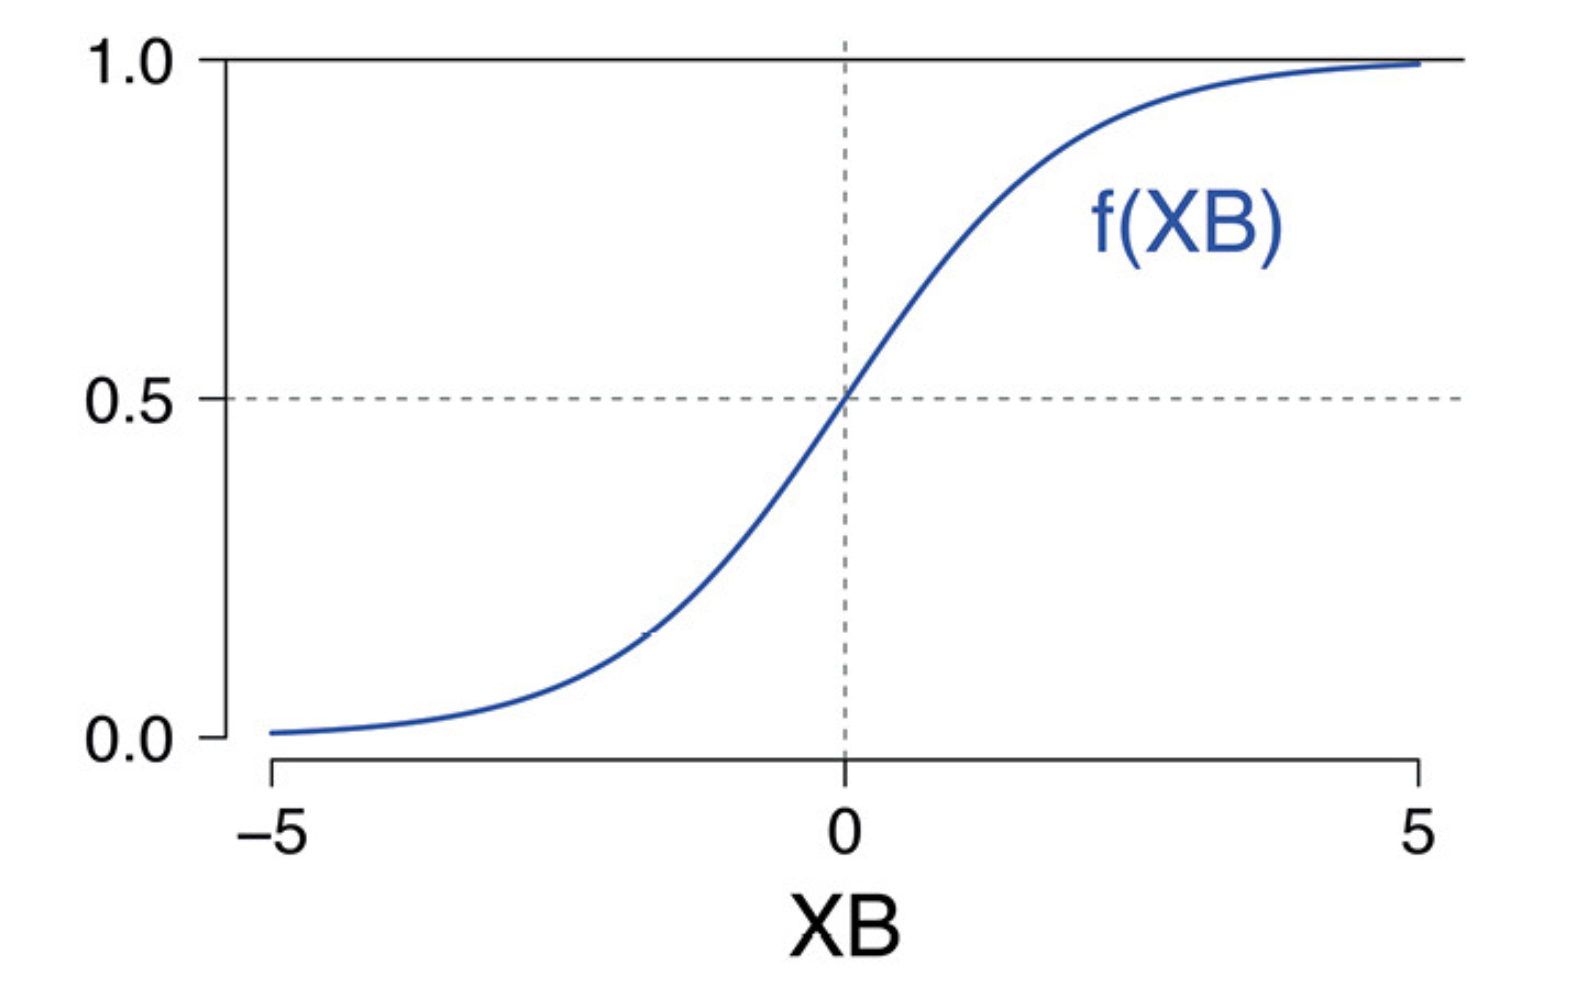
\includegraphics[scale=0.2]{figures/logistic}
              \\
              \tiny
              Source: Taddy (2019)
 \end{figure}

\end{frame}
%----------------------------------------------------------------------%
\begin{frame}[fragile]
\frametitle{Logit}
  \begin{itemize}


    \item Tenemos la probabilidad condicional
    \begin{align}
    Pr(y=1|X) &= f(X'\beta) 
    \end{align}
    \item Estimamos los parámetros usando MLE
    \medskip
    \item Podemos recobrar fácilmente las predicciones:
  \end{itemize}


\begin{align}
p(y=1|X)=\frac{exp(\hat{\beta}_0 +\hat{\beta}_1 x_1 + \dots +\hat{\beta}_p x_p)}{1+exp(\hat{\beta}_0 +\hat{\beta}_1 x_1 + \dots +\hat{\beta}_p x_p)}
\end{align}

\end{frame}
%----------------------------------------------------------------------%
\begin{frame}[fragile]
\frametitle{ROC}


\begin{columns}[T] % align columns
\begin{column}{.52\textwidth}
\begin{itemize}
\item ROC ilustra el trade-off de las reglas de clasificación
\medskip
\item ROC nos da el $locus $ de los $TPR$ y $FPR$ para todos los posibles $c\in[0,1]$
  \begin{itemize}
    \item {\it Sensibilidad:} Tasas de Verdaderos Positivos
    \item {\it 1-Especificidad:} Tasa de Falsos Positivos
    
  \end{itemize}
\item Nos da la habilidad
\begin{itemize}
  \item Medir la capacidad predictiva del modelo
  \medskip
  \item $\,$
  \medskip
\end{itemize}
\end{itemize}
\end{column}  
\hfill
\begin{column}{.48\textwidth}

 \begin{figure}[H] \centering
            \captionsetup{justification=centering}
              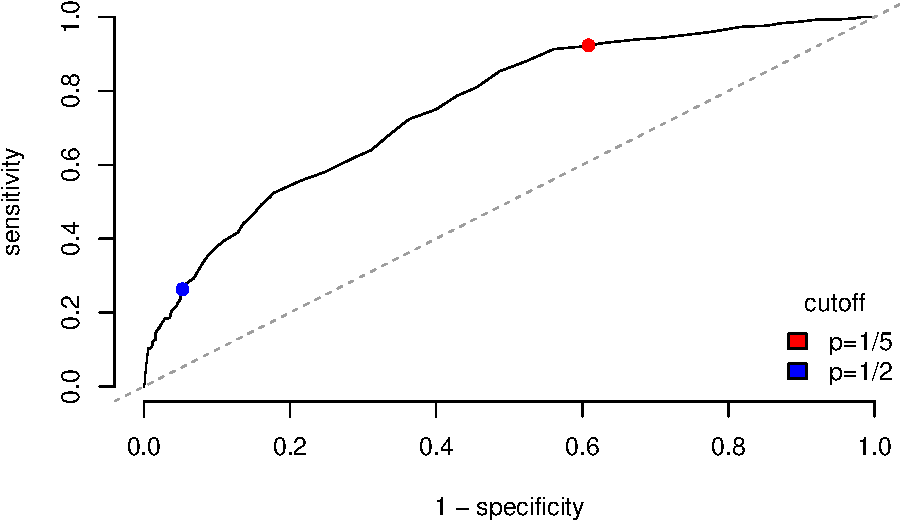
\includegraphics[scale=0.4]{figures/roc}                            
 \end{figure}

\end{column}
\end{columns}


\end{frame}
%----------------------------------------------------------------------%
\begin{frame}[fragile]
\frametitle{ROC}



\begin{columns}[T] % align columns
\begin{column}{.52\textwidth}
\begin{itemize}
\item ROC ilustra el trade-off de las reglas de clasificación
\medskip
\item ROC nos da el $locus $ de los $TPR$ y $FPR$ para todos los posibles $c\in[0,1]$
  \begin{itemize}
    \item {\it Sensibilidad:} Tasas de Verdaderos Positivos
    \item {\it 1-Especificidad:} Tasa de Falsos Positivos
    
  \end{itemize}
\item Nos da la habilidad
\begin{itemize}
  \item Medir la capacidad predictiva del modelo
  \medskip
  \item Comparar entre modelos
  
\end{itemize}
\end{itemize}
\end{column}  
\hfill
\begin{column}{.48\textwidth}

 \begin{figure}[H] \centering
            \captionsetup{justification=centering}
              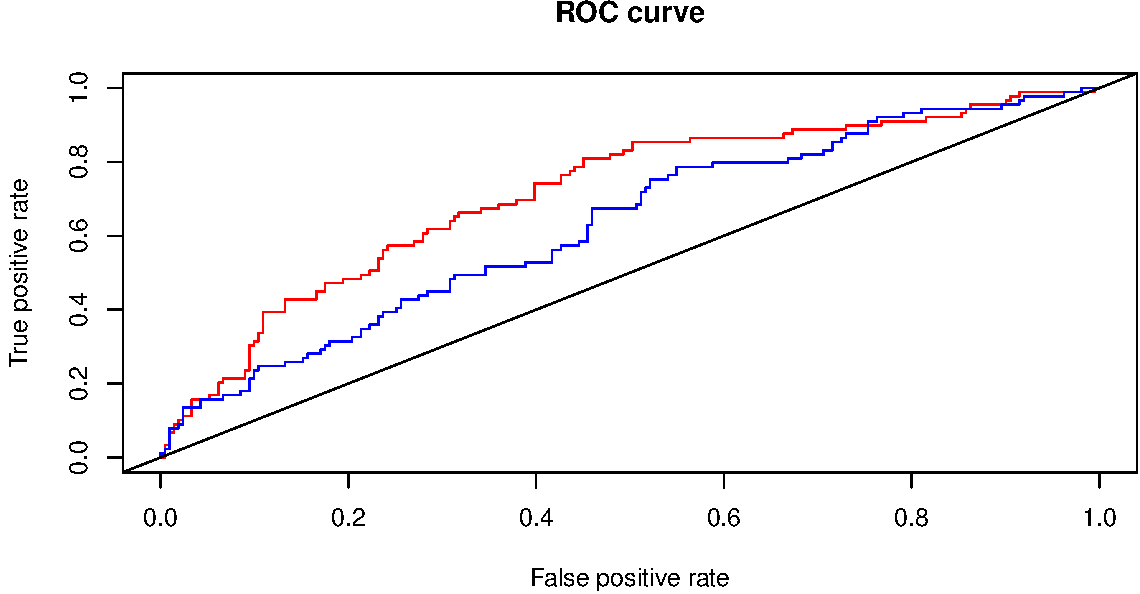
\includegraphics[scale=0.38]{figures/unnamed-chunk-11-1.pdf}
 \end{figure}

\end{column}
\end{columns}



\end{frame}

%----------------------------------------------------------------------%
\begin{frame}
\frametitle{Revisión }
  
Hoy
    \medskip
    \begin{itemize} 
        \item Regularización
         \medskip
         \begin{itemize}  
           \item Lasso 
           \medskip
           \item Ridge
        \end{itemize}   
         \item Clasificación
         \medskip
        \begin{itemize}  
           \item Vecinos Cercanos
           \medskip
           \item Logit
           \medskip
           \item ROC
        \end{itemize}
    \end{itemize}
  





\end{frame}

%----------------------------------------------------------------------%
\section{Break}
\begin{frame}
\frametitle{}

\begin{centering}
\huge
\textcolor{andesred}{Volvemos en 5 mins con \texttt{R} }

\end{centering}

\end{frame}
%----------------------------------------------------------------------%
\section{\texttt{R para ML}}
%----------------------------------------------------------------------%
\begin{frame}
\frametitle{R para ML}

\begin{figure}[H] \centering
  \centering
  
\includegraphics[scale=0.35]{figures/baticomputer_meme.jpg}
  \\
  \tiny photo from \url{https://www.dailydot.com/parsec/batman-1966-labels-tumblr-twitter-vine/}
\end{figure}

\end{frame}
%----------------------------------------------------------------------%
%----------------------------------------------------------------------%
\end{document}
